\documentclass[aspectratio=169]{beamer}
%\documentclass[handout]{beamer}

% \usepackage{ensislidesOG}
%\usepackage[utf8]{inputenc}
% \usepackage[T1]{fontenc}
\usepackage[english]{babel}

\usepackage{amsfonts}
\usepackage{amsmath}
\usepackage{amssymb}
\usepackage{amsthm}
% \usepackage[frenchstyle]{mathalpha}
% \usepackage[OMLmathsfit]{isomath}
\usepackage{graphicx}
\usepackage{color} % for ps_tex inclusions
\usepackage{fmtcount} % th, e.g. \ordinalnum{4}
\usepackage{booktabs}
\usepackage{xmpmulti}
\usepackage{multimedia}

\usetheme{Boadilla}
\usecolortheme{crane}

\newcommand{\itb}{\item[$\bullet$]}
\newcommand{\dps}{\displaystyle}

\def\<{{\guillemotleft}}
\def\>{{\guillemotright}}

\def\vs1{\vspace{1mm}}
\def\v3{\vspace{3mm}}

\newcommand{\II}{\,\mbox{I\hskip -0.600em 1}}

\newcommand{\ME}{{\mathcal E}}
\newcommand{\MN}{{\mathcal N}}

\newcommand{\NN}{\ensuremath{\mathbb{N}}}
\newcommand{\RR}{\ensuremath{\mathbb{R}}}

\newcommand{\card}{\mbox{card}}
\newcommand{\pa}{\mbox{pa}}

\newcommand{\De}{\mbox{De}}
\newcommand{\Nd}{\mbox{Nd}}
\newcommand{\Ne}{\mbox{Ne}}
\newcommand{\vect}[1]{\mathbf{#1}}

\newcommand{\indep}{\perp\!\!\!\perp}
\newcommand{\condindep}[3]{#1 \indep #2 \vert #3}
\newcommand{\condindepP}[4]{#1 \indep_{#4} #2 \vert #3}
\newcommand{\ts}[3]{#1_{#2}^{#3}}
\newcommand{\set}[1]{\{#1\}}

\newcommand{\centerimage}[2]{\begin{center}\includegraphics[width=#1\textwidth]{#2}\end{center}}

\usepackage{tikz}
\usetikzlibrary{decorations.pathmorphing,decorations.text} % noisy shapes
\usetikzlibrary{fit}					% fitting shapes to coordinates
\usetikzlibrary{backgrounds,intersections}	% drawing the background after the foreground
\usetikzlibrary{positioning,calc,matrix}


\title[ALM]{Advanced Machine Learning\\ Applications to Vision, Audio \& Text}

\subtitle{Introduction, Basics, Deep Learning} % (optional)

\author[Xavi]{Xavier Alameda-Pineda}
% - Use the \inst{?} command only if the authors have different
%   affiliation.

\institute{MSIAM/MoSIG -- 2024-2025}


\makeatother
\setbeamertemplate{footline}
{
  \leavevmode%
%   \hbox{%
%   \begin{beamercolorbox}[wd=.4\paperwidth,ht=2.25ex,dp=1ex,center]{author in head/foot}%
%     \usebeamerfont{author in head/foot}\insertshortauthor
%   \end{beamercolorbox}%
%   \begin{beamercolorbox}[wd=.6\paperwidth,ht=2.25ex,dp=1ex,center]{title in head/foot}%
    \usebeamerfont{title in head/foot}\hfill
    \insertframenumber{} / \inserttotalframenumber\hspace*{1ex}
%   \end{beamercolorbox}}%
%   \vskip0pt%
}
\makeatletter
\setbeamertemplate{navigation symbols}{}

\AtBeginSection[]{
  \begin{frame}
  \vfill
  \centering
  \begin{beamercolorbox}[sep=8pt,center,shadow=true,rounded=true]{title}
    \usebeamerfont{title}\insertsectionhead\par%
  \end{beamercolorbox}
  \vfill
  \end{frame}
}

\date{}

%%%%%%%%%%%%%%%%%%%%%%%%%%%%%%%%%%%%%%%%%%%%%%%%%%%%%%%%%%%%%%

\begin{document}

\begin{frame}
  \titlepage
\end{frame}


% %%%%%%%%%%%%%%%%%%%%%%%%%%%%%%%%%%%%%%%%%%%%%%%%%%%%%%%%%%%%%%
% \section{Course Organisation}
% %%%%%%%%%%%%%%%%%%%%%%%%%%%%%%%%%%%%%%%%%%%%%%%%%%%%%%%%%%%%%%

% \begin{frame}{Course Motivation}
% This course was previously known as:
% \begin{itemize}
%  \item Category Learning and Object Recognition
%  \item ML for Computer Vision and Audio Processing
%  \item Machine Learning for Multimodal Data
% \end{itemize}\vspace{3mm}
% 
% Why changing? 
% \begin{itemize}
%  \item Research topics in these areas are evolving
%  \item To study different modalities and their interactions
%  \item Broadens the spectrum for applications
%  \item More up-to-date content
% \end{itemize}
% 
% \end{frame}


\begin{frame}{AML Team Upcoming Lectures}
 \begin{columns}
  \begin{column}{0.1\textwidth}
  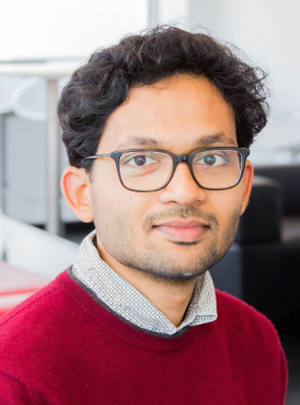
\includegraphics[width=\textwidth]{images/karteek.jpg} 
  \end{column}
  \begin{column}{0.7\textwidth}
  \textbf{Karteek Alahari}\\
   Director of Research [\alert{\href{https://lear.inrialpes.fr/people/alahari/}{website}}] @inthebrownbag\\
    THOTH Team, Inria @ UGA\\
    Machine learning for computer vision, big visual data.
  \end{column}
 \end{columns}\vspace{3mm}
% \end{frame}
%
% \begin{frame}{ALM Team: Pia Bideau}
 \begin{columns}
  \begin{column}{0.1\textwidth}
  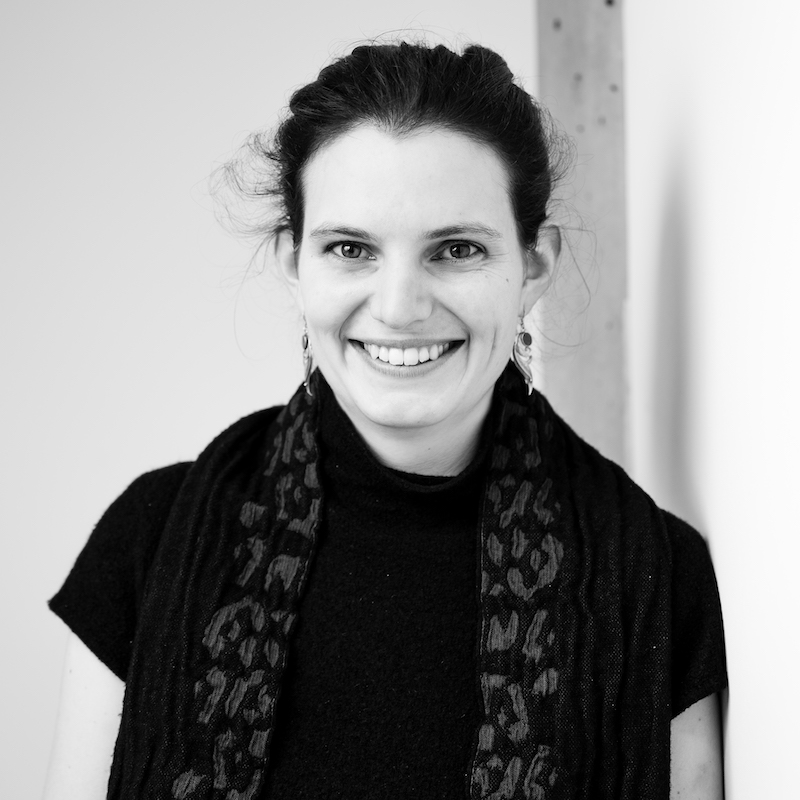
\includegraphics[width=\textwidth]{images/pia.jpg}
  \end{column}
  \begin{column}{0.7\textwidth}
  \textbf{Pia Bideau}\\
   Research Scientist [\alert{\href{https://www.user.tu-berlin.de/pbideau/}{website}}]\\
    THOTH Team, Inria @ UGA\\
    Computer vision, robotics.
  \end{column}
 \end{columns}\vspace{3mm}
% \end{frame}
%
% \begin{frame}{ALM Team: Xavier Alameda-Pineda (Xavi)}
 \begin{columns}
  \begin{column}{0.1\textwidth}
  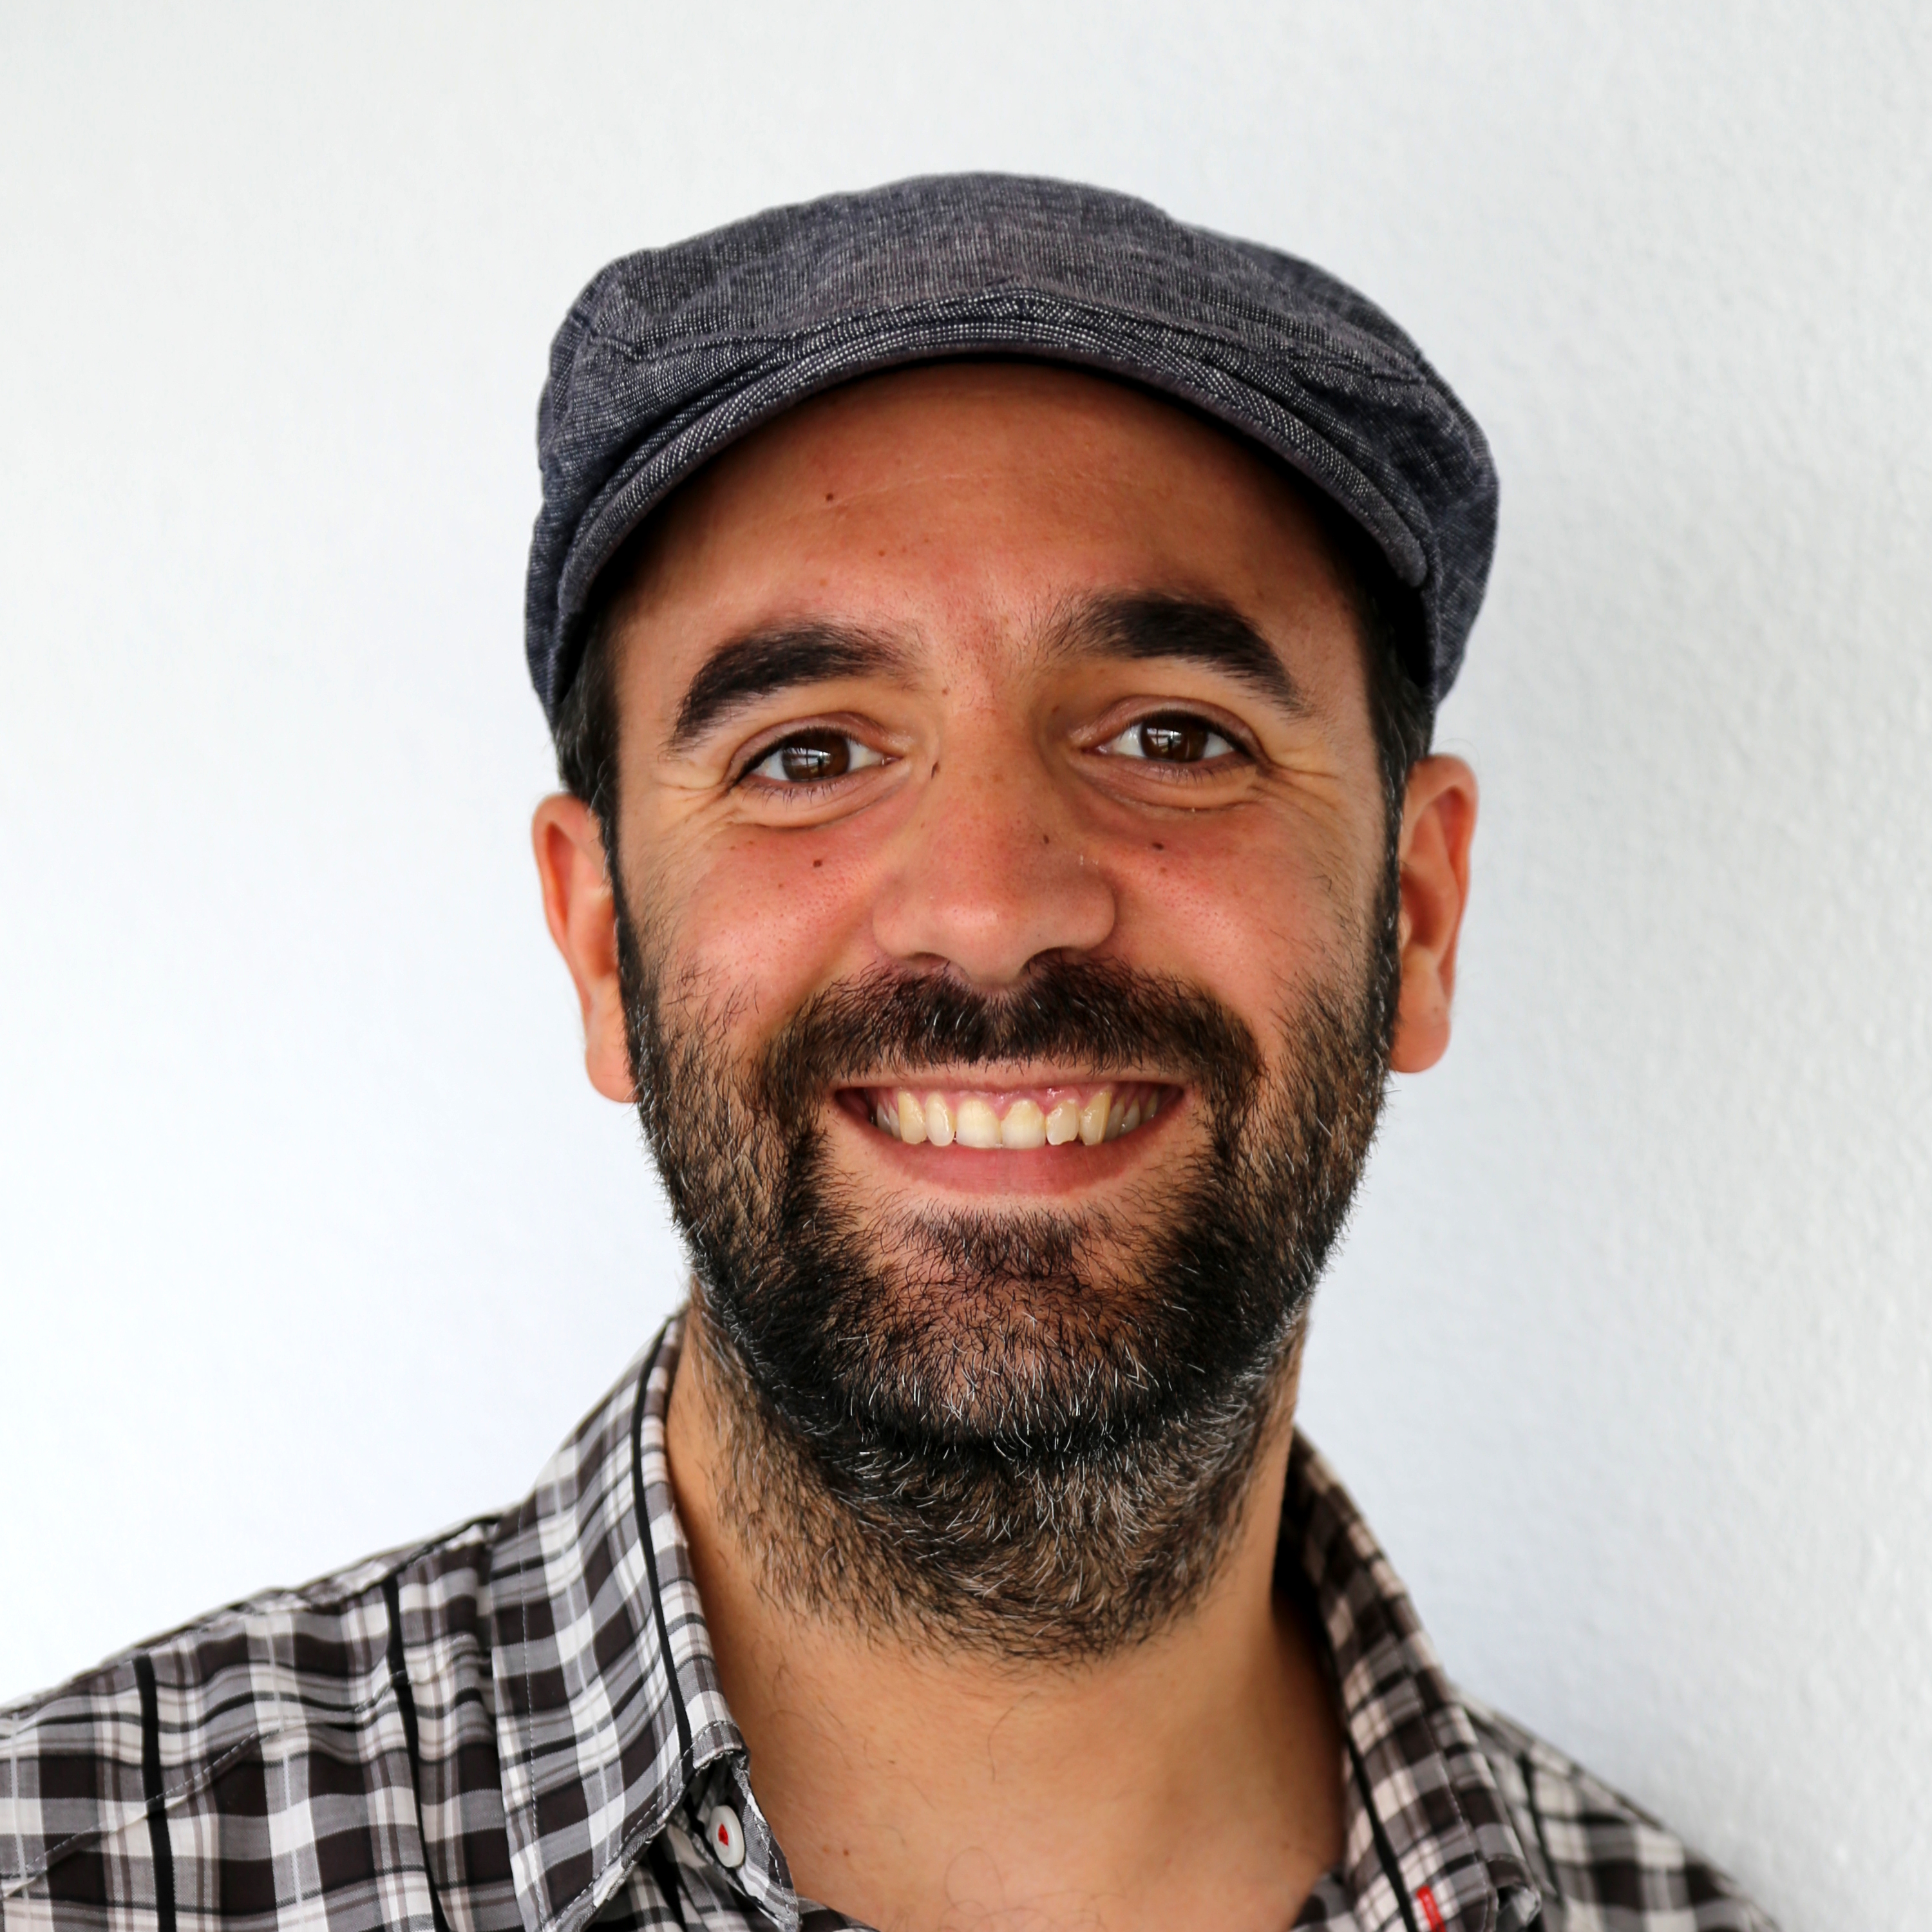
\includegraphics[width=\textwidth]{images/xavi-square.jpg} 
  \end{column}
  \begin{column}{0.7\textwidth}
  \textbf{Xavier Alameda-Pineda} (Xavi)\\
   Director of Research [\href{http://xavirema.eu}{\alert{website}}] @xavirema\\
   RobotLearn Team, Inria @ UGA\\
   AV perception, probabilistic and deep learning, HRI.
  \end{column}
 \end{columns}\vspace{4mm}
 Email: \texttt{name.lastname@inria.fr}
\end{frame}


\begin{frame}{Course Organisation}
 Final grade: 0.5*FE + 0.5*ME
 \begin{itemize}
  \item Final Exam (FE)
  \item Mid-term Exam (ME)
 \end{itemize}\vspace{4mm}
 
 Regarding the Paper Presentations:
 \begin{itemize}
  \item 12 papers presented in two sessions (20/12 \& 10/01)
  \item FE: Course content + papers content
  \item \textbf{Bonus} for the presenters
  \item Send an e-mail with your choice\textbf{\alert{S}} to Karteek AND myself.
 \end{itemize}\vspace{4mm}
 
 All materials in Chamilo.
 
\end{frame}


\begin{frame}{Modalities}
\centering
 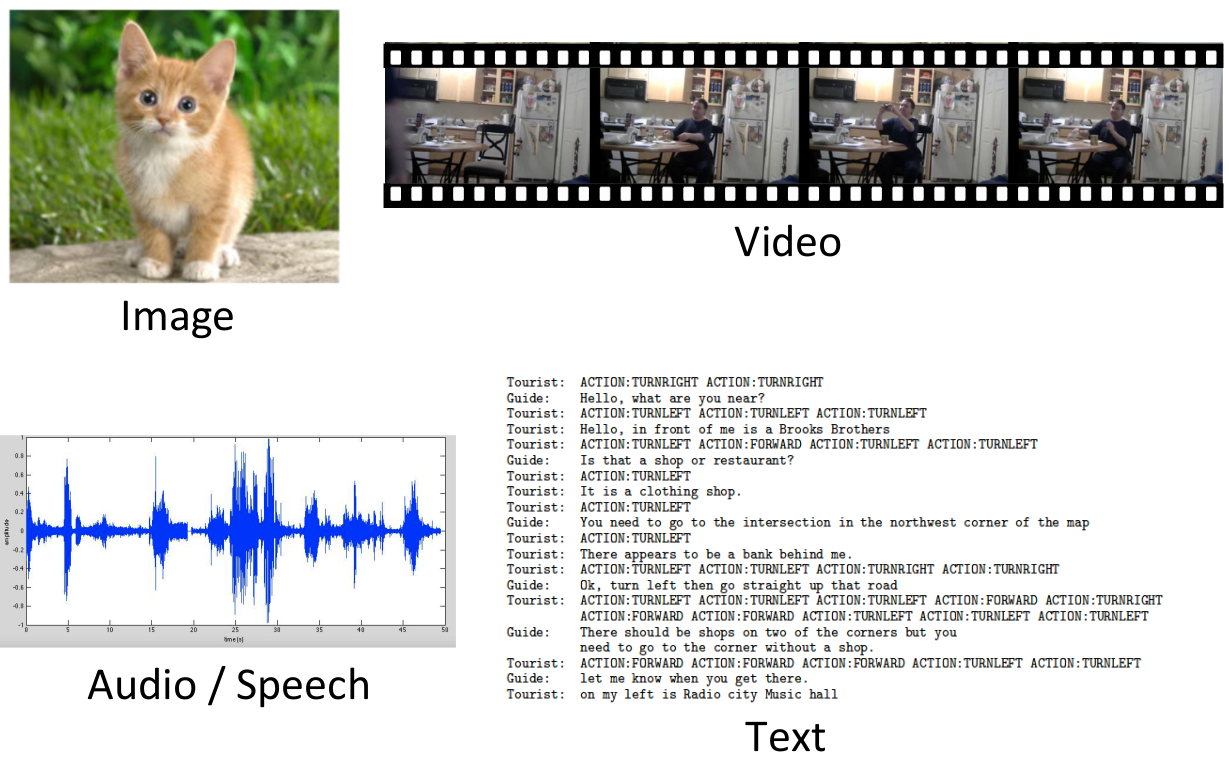
\includegraphics[width=0.8\textwidth]{images/modalities.png}
\end{frame}



\begin{frame}{Schedule}
\centering
 \begin{tabular}{ccc}
  \toprule
  When? & What? & Who? \\
  \midrule
  8-Nov & Intro, DL Recap, Conv, ... & Xavi \\
  15-Nov & Exam & Eric \\
  22-Nov & Attention, Audio, Audio-Visual & Xavi \\
  29-Nov & \alert{No class}\\
  06-Dec & Visual Data & Pia \\
  13-Dec & Video, GAN & Karteek \\
  20-Dec & Paper presentation 1 & Xavi \\
  10-Jan & Paper Presentation 2 & Karteek \\
  \bottomrule
 \end{tabular}
\end{frame}

\begin{frame}{Applications: classification, localisation, segmentation, ...}
 \begin{figure}
  \centering
  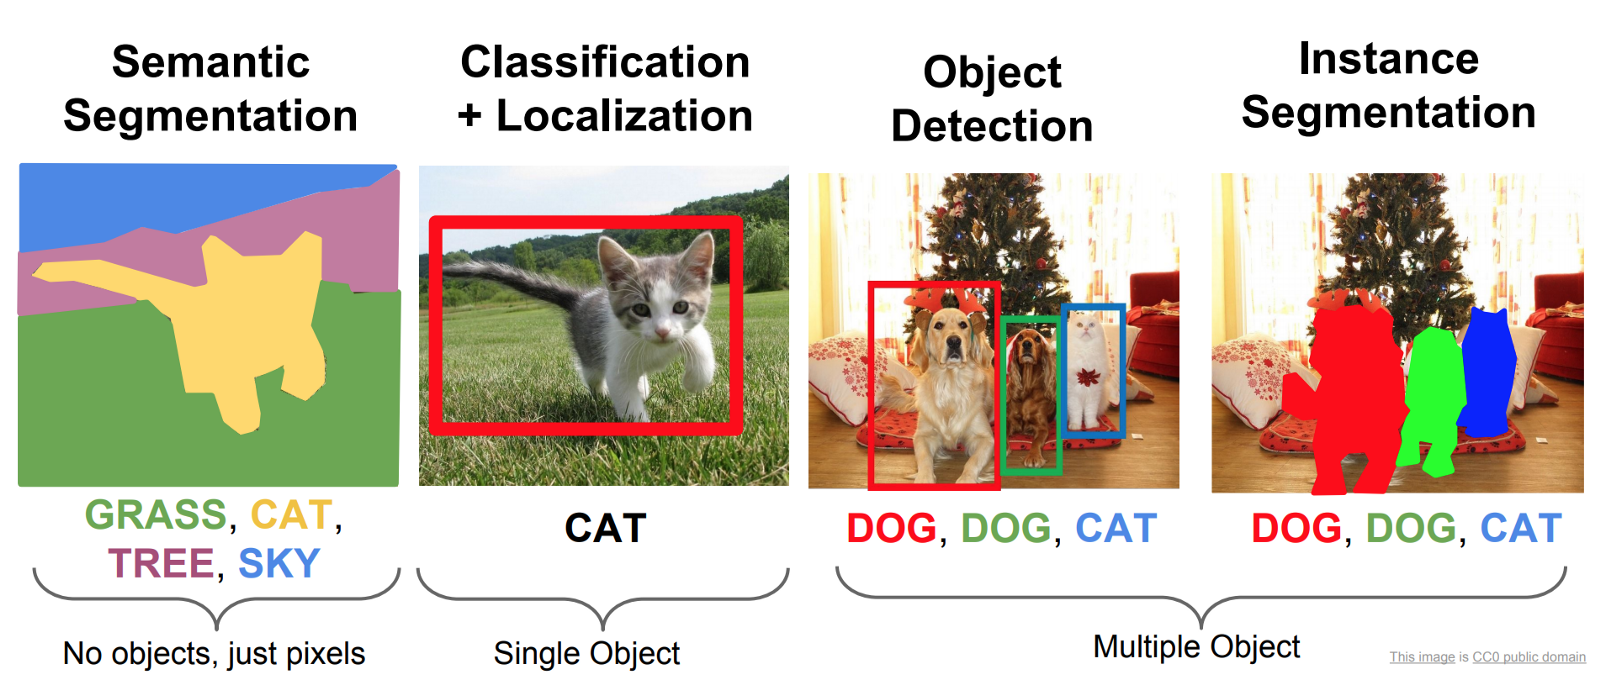
\includegraphics[width=0.9\textwidth]{images/instancesegmentation}
 \end{figure}
\end{frame}
%
% \begin{frame}{Applications: Object detection}
%  Object detection: find all objects and their category in an image.\\
%  \begin{figure}
%   \centering
%   \includegraphics[height=4cm]{images/objectdetection1}
%   \hspace{4mm}
%   \includegraphics[height=4cm]{images/objectdetection2}
%  \end{figure}
% Challenges: unknown number of objects, occlusions, appearance changes.
% \end{frame}
%
% \begin{frame}{Applications: Semantic segmentation}
%  Semantic segmentation: infer a class label for each pixel in the image.\\
%  \begin{figure}
%   \centering
%    \includegraphics[height=2.8cm]{images/semanticsegmentation1}
%    \hspace{4mm}
%    \includegraphics[height=2.8cm]{images/semanticsegmentation2}
%  \end{figure}
% \end{frame}

%
% \begin{frame}{Applications: Instance segmentation}
%  Instance segmentation: map each pixel to an instance of an object.\\
%  \begin{figure}
%   \centering
%   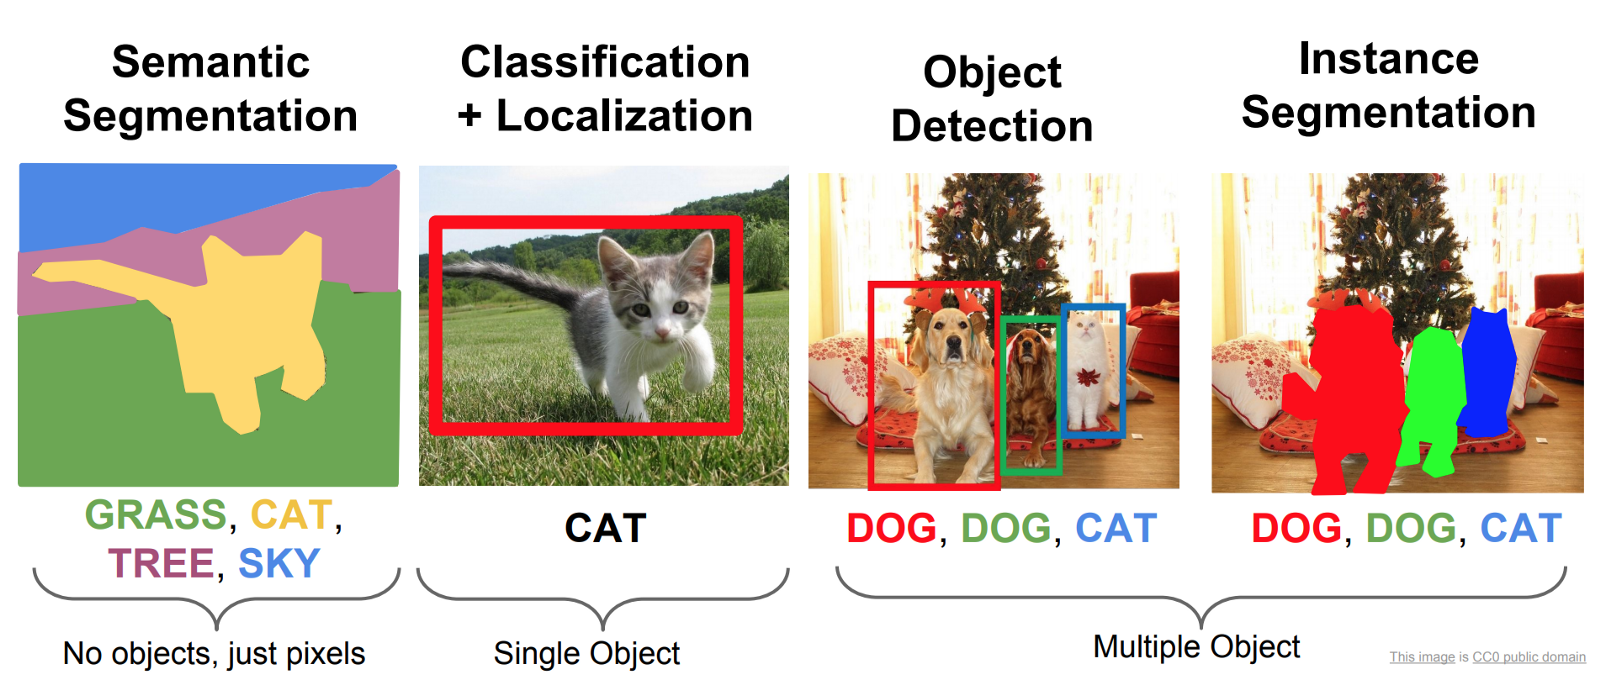
\includegraphics[width=0.8\textwidth]{images/instancesegmentation}
%  \end{figure}
% \end{frame}

\begin{frame}{Applications: Image translation}
 \begin{figure}
  \centering
  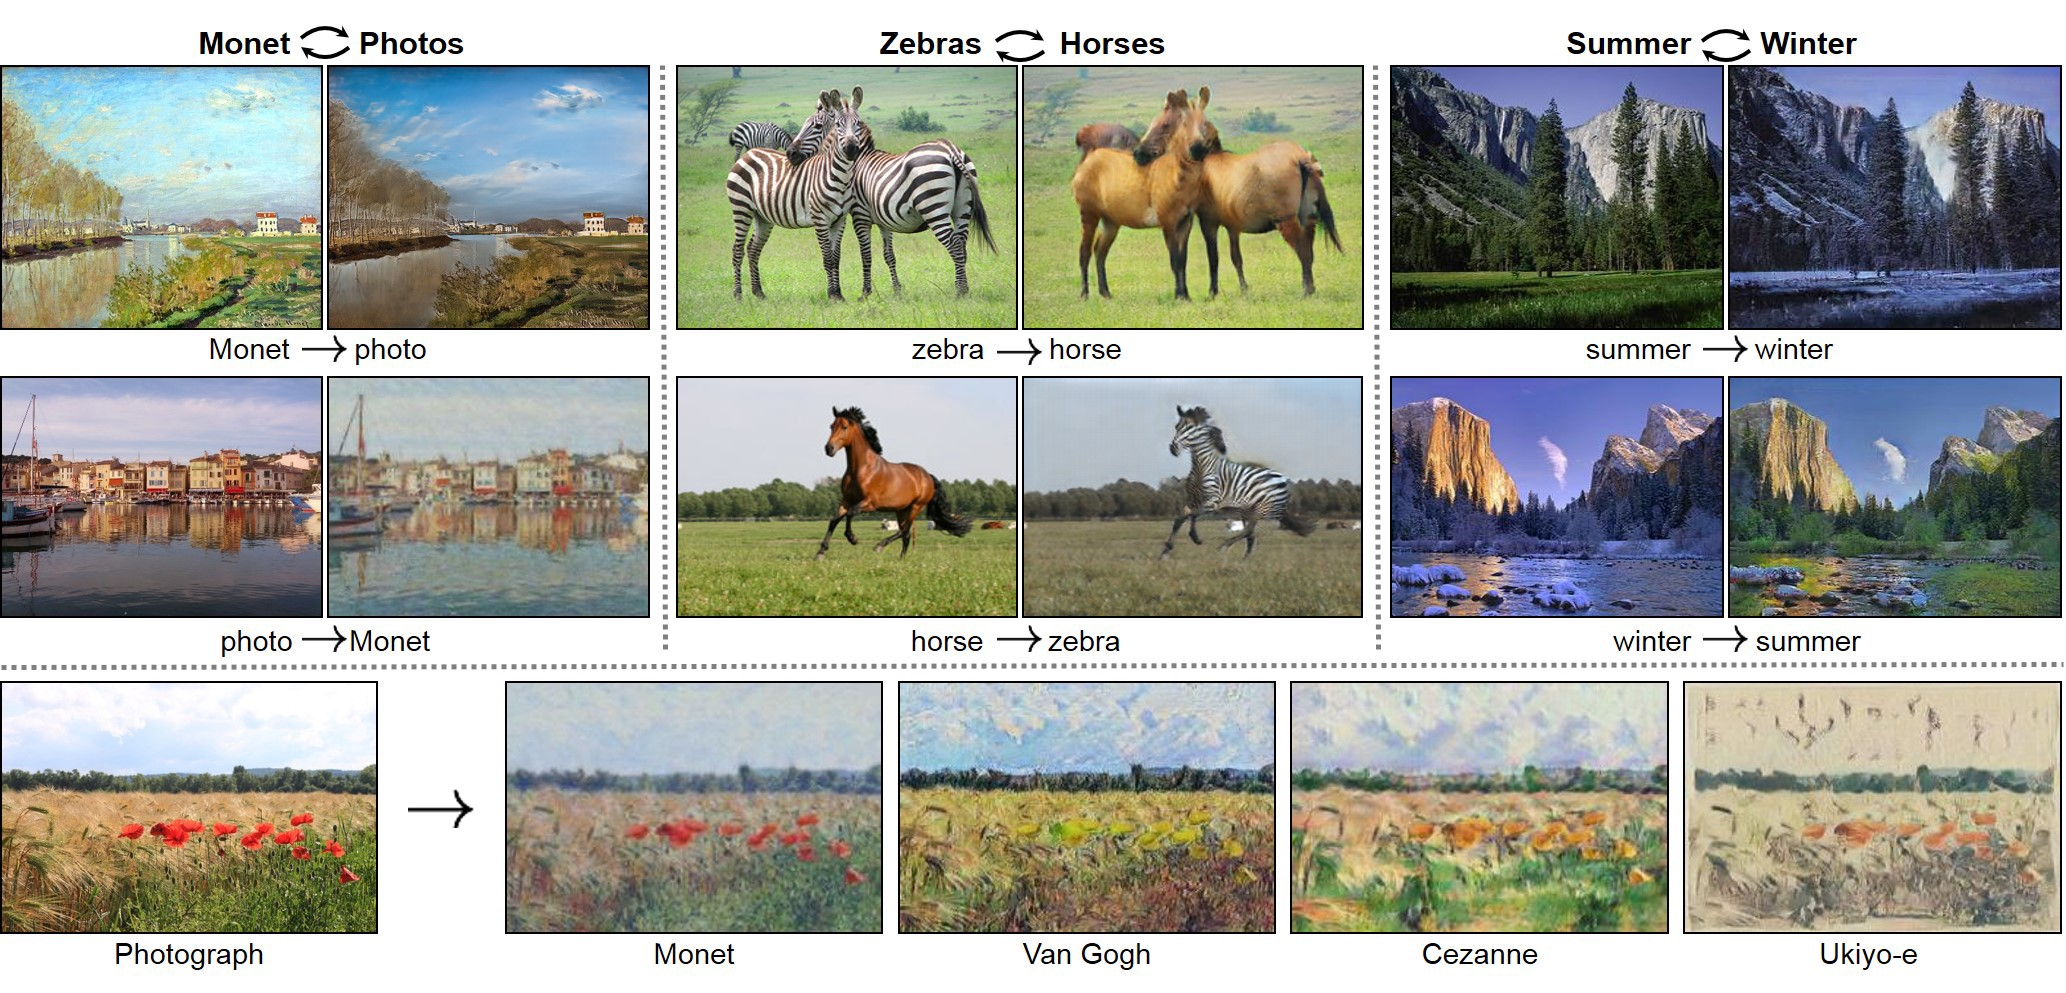
\includegraphics[width=\textwidth]{images/imagetranslation}
 \end{figure}
\end{frame}

\begin{frame}{Applications: Captioning}
 \begin{figure}
  \centering
  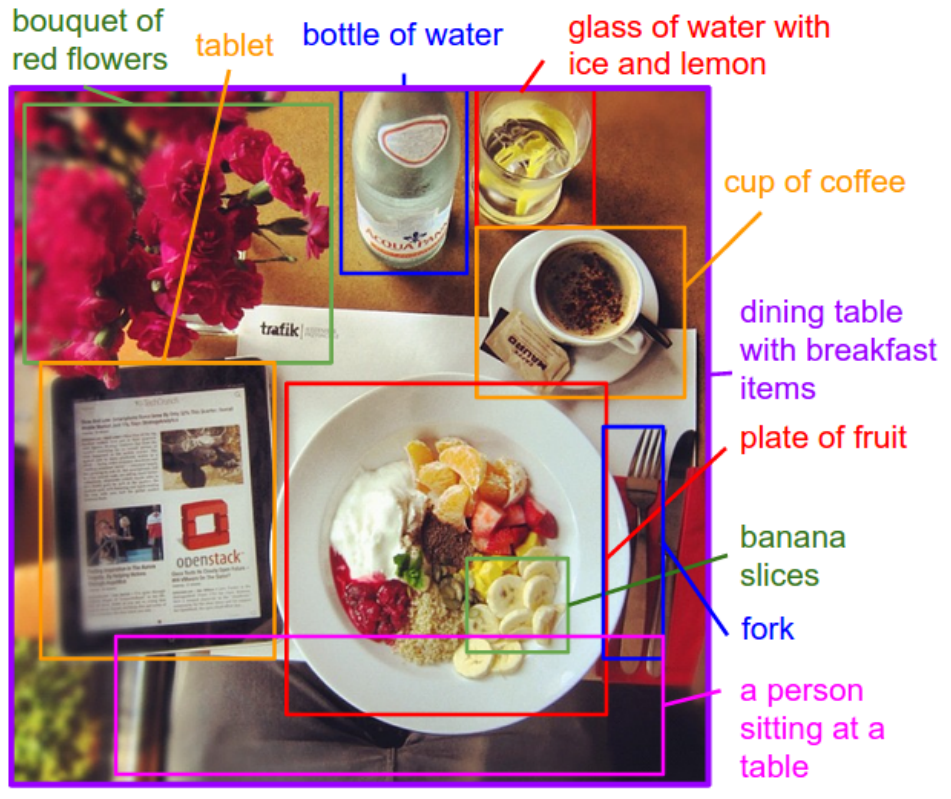
\includegraphics[width=0.6\textwidth]{images/Captioning}
 \end{figure}
\end{frame}

\begin{frame}{Applications: Visual question answering}
 \begin{figure}
  \centering
  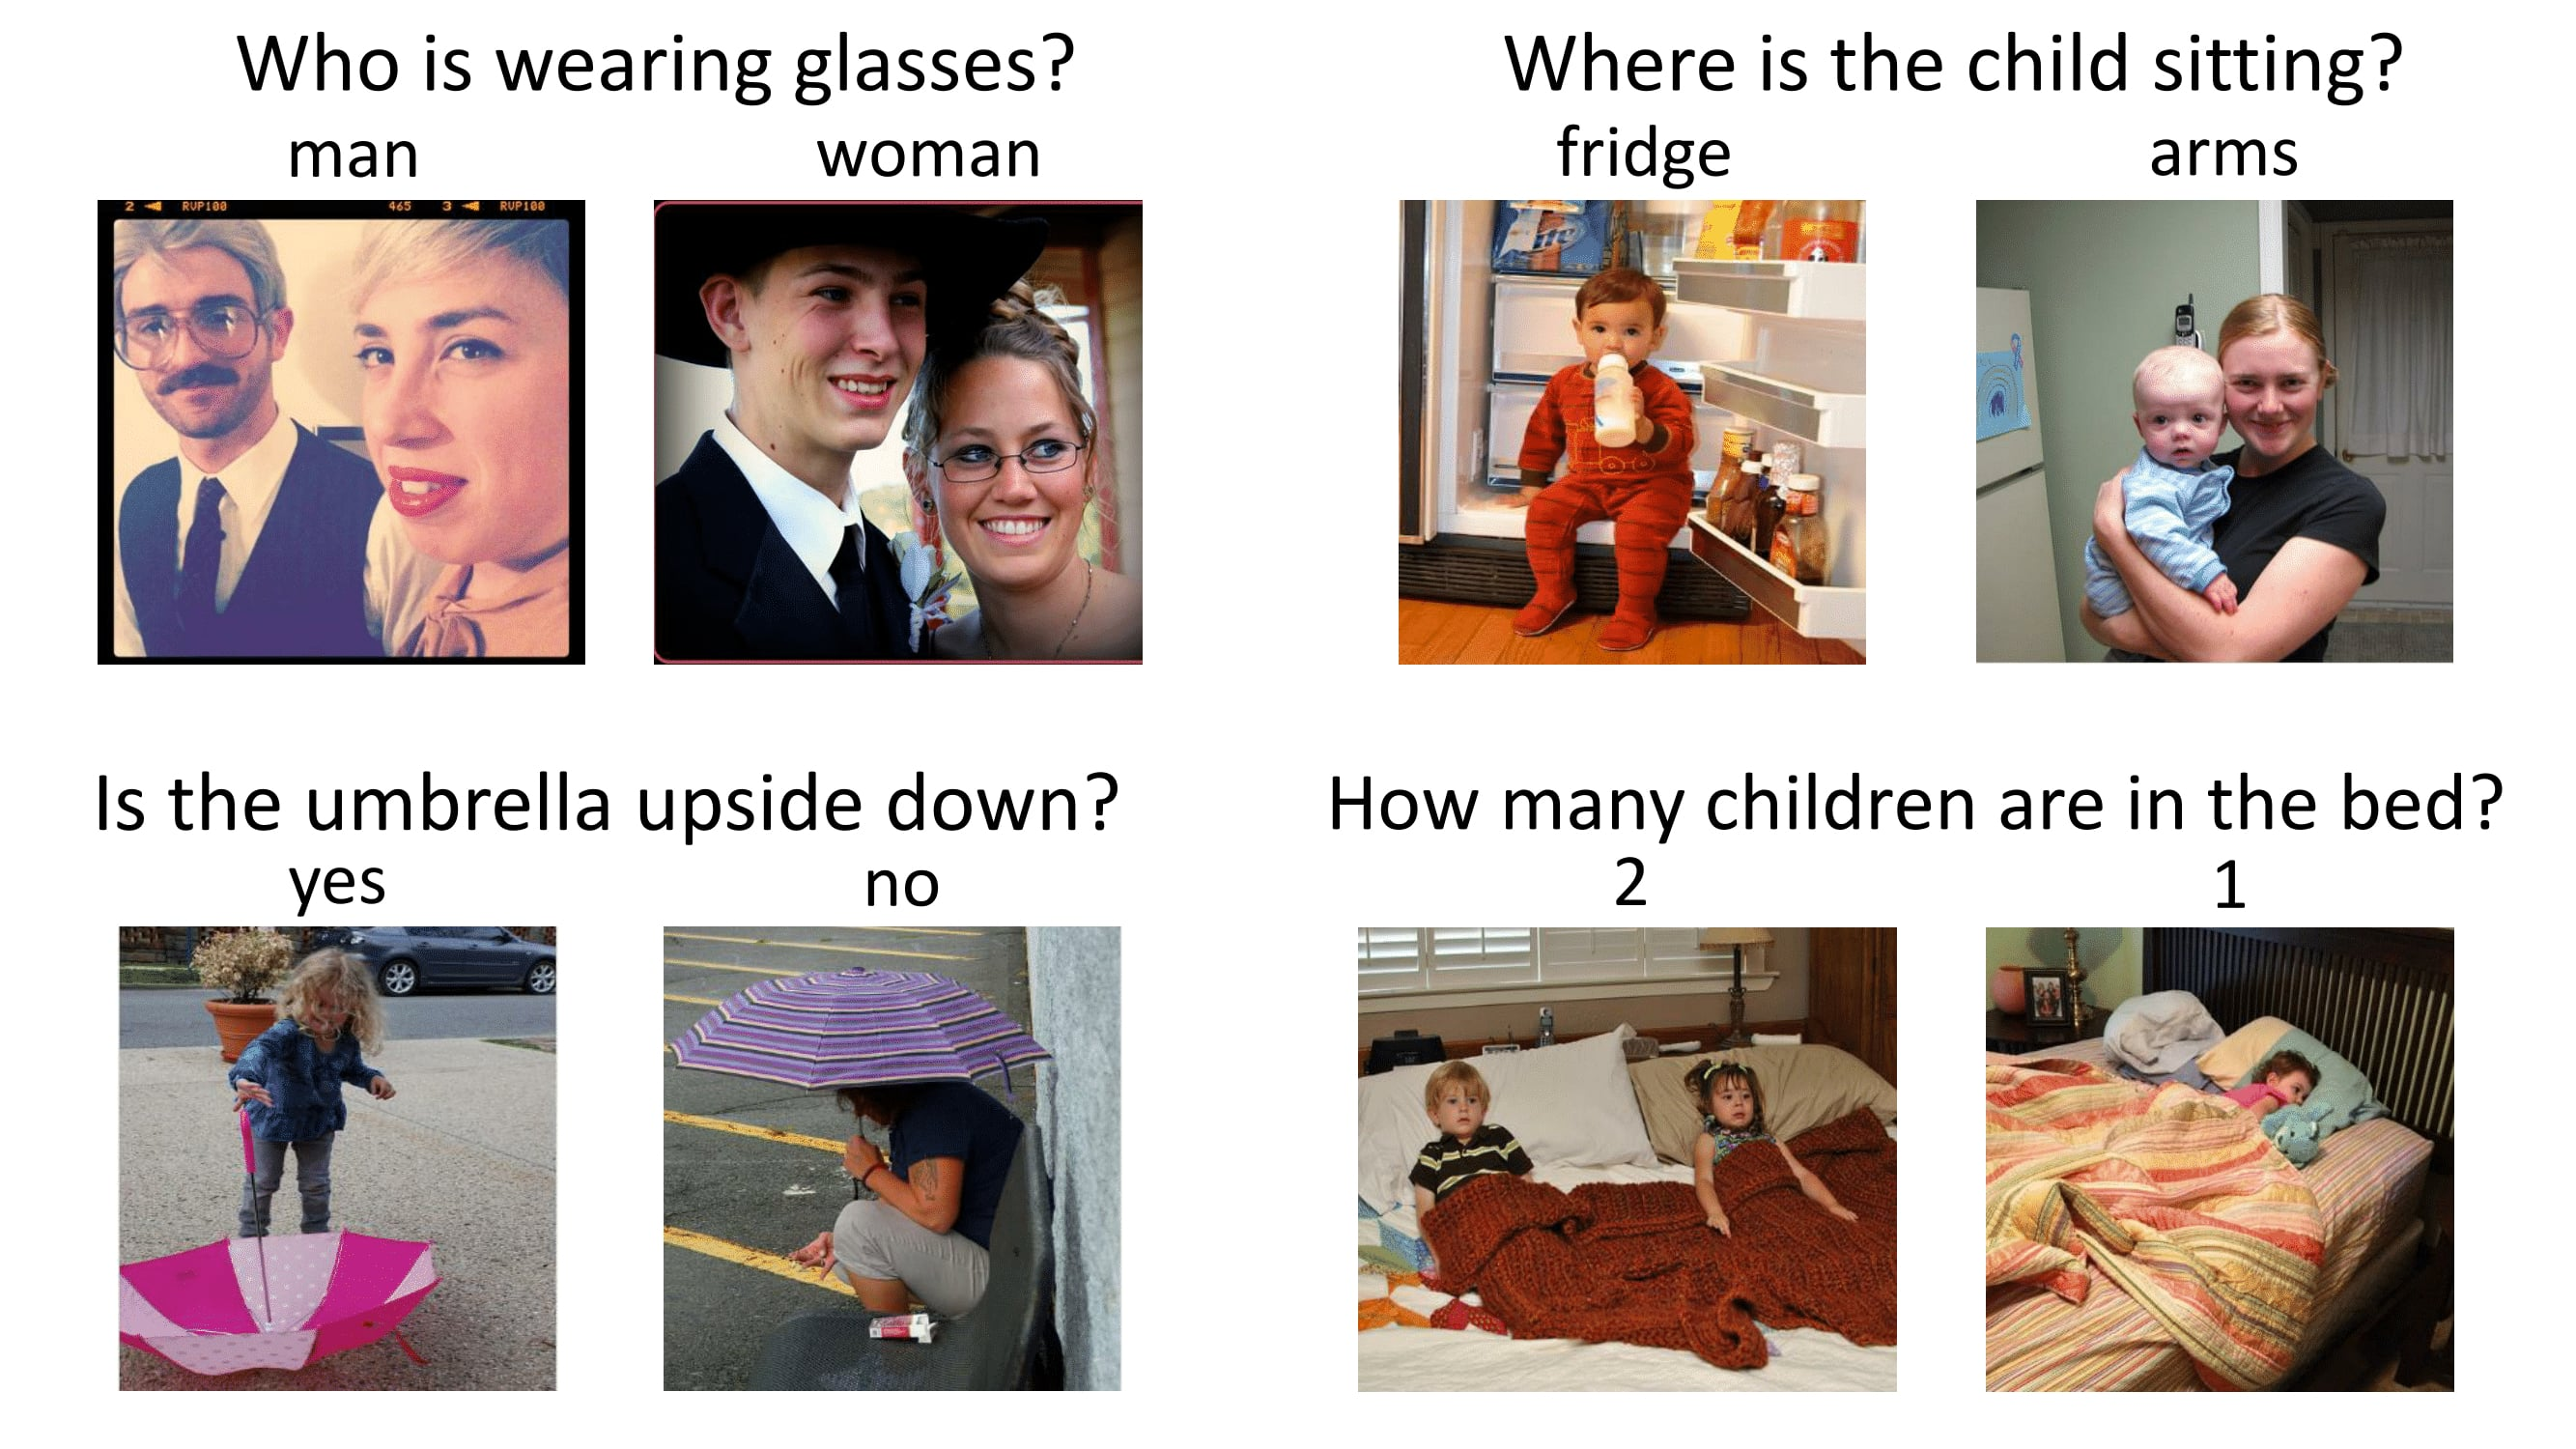
\includegraphics[width=0.8\textwidth]{images/vqa}
 \end{figure}
\end{frame}

\begin{frame}{Applications: Object tracking}
Following objects/persons through time.\vspace{4mm}
 \begin{figure}
  \centering
  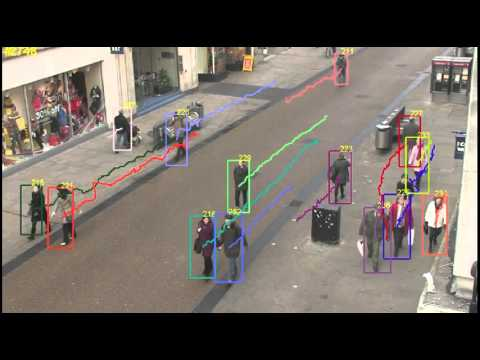
\includegraphics[width=0.4\textwidth]{images/tracking1}\hspace{4mm}
  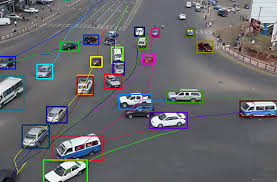
\includegraphics[width=0.4\textwidth]{images/tracking2}
 \end{figure}
\end{frame}
%
% \begin{frame}{Applications: Person re-identification}
%  Find the same person in another camera.\vspace{4mm}
%  \begin{figure}
%   \centering
%   \includegraphics[width=\textwidth]{images/personreid}
%  \end{figure}
% \end{frame}
%
% \begin{frame}{Applications: Lip reading}
% \begin{figure}
%   \centering
%   \includegraphics[width=0.9\textwidth]{images/lipreading}
%  \end{figure}
%  Be careful: not all speech can be seen.
% \end{frame}
%
%
%
% \begin{frame}{Applications: Acoustic scene classification}
%  \begin{figure}
%   \centering
%   \includegraphics[width=0.7\textwidth]{images/acousticsceneclassification}
%  \end{figure}
% \end{frame}

\begin{frame}{Applications: Audio segmentation}
 \begin{figure}
  \centering
  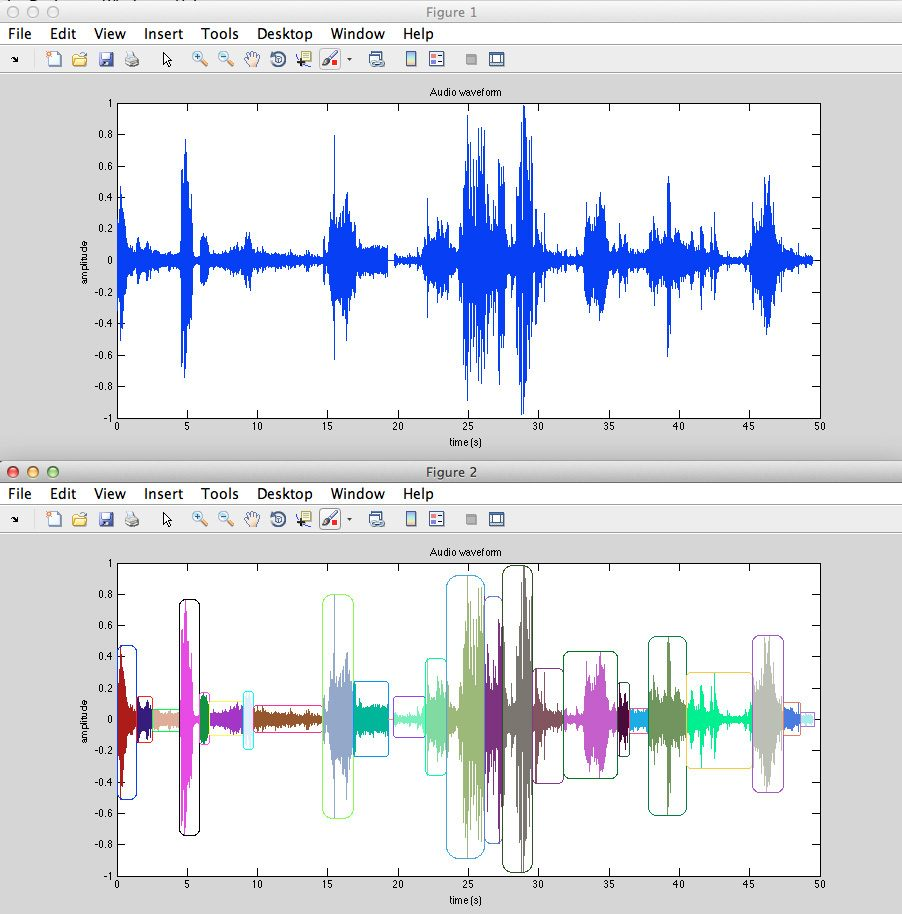
\includegraphics[width=0.5\textwidth]{images/audiosegmentation}
 \end{figure}
\end{frame}

% \begin{frame}{Applications: Audio event segmentation and classification}
%  \begin{figure}
%   \centering
%   \includegraphics[width=0.5\textwidth]{images/audioeventclassification}
%  \end{figure}
%  The terminology is different than in the visual case. In audio we say \textit{segmentation} rather than \textit{localisation}, and we use \textit{event} rather than \textit{instance}.
% \end{frame}

\begin{frame}{Applications: Sound source localisation}
 \begin{figure}
  \centering
  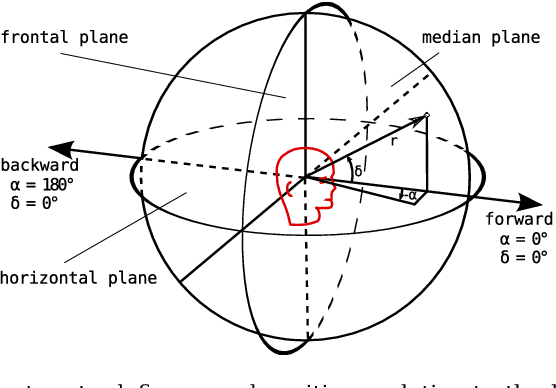
\includegraphics[width=0.4\textwidth]{images/soundlocalisation1}\hspace{4mm}
  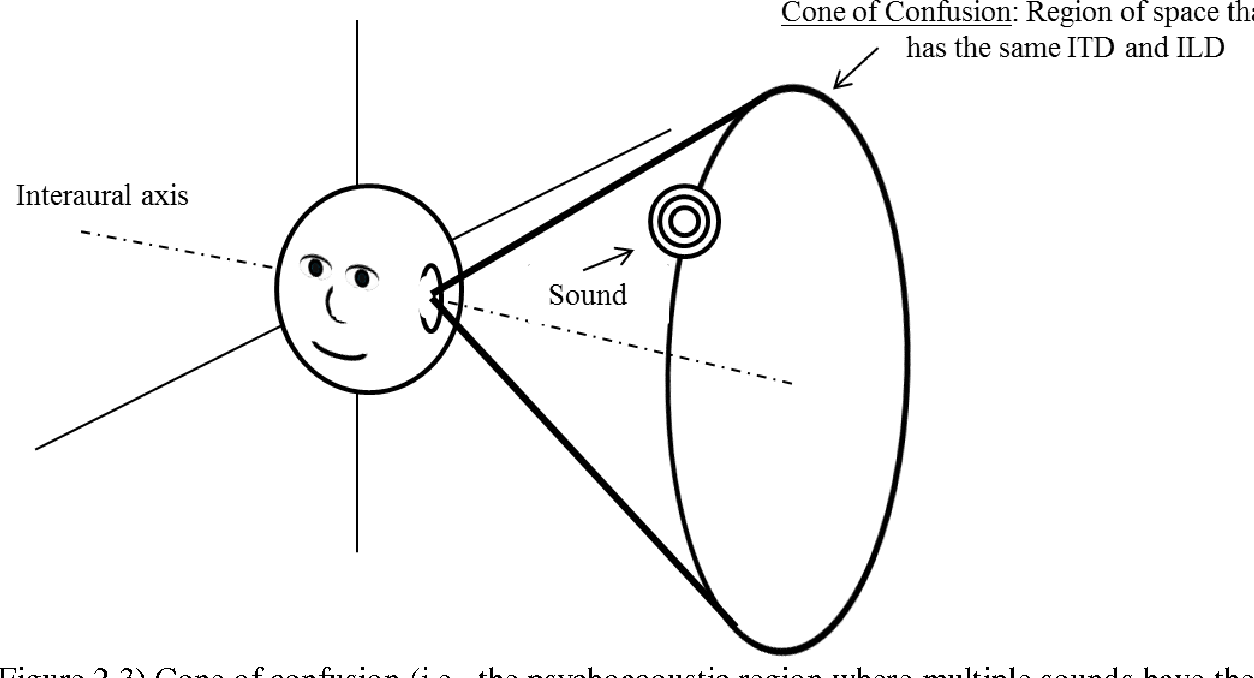
\includegraphics[width=0.4\textwidth]{images/soundlocalisation2}
 \end{figure}
\end{frame}

\begin{frame}{Applications: Sound source separation}
 \begin{figure}
  \centering
  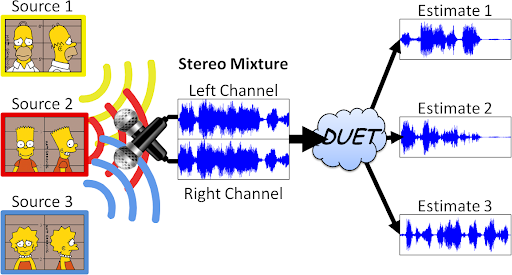
\includegraphics[width=0.8\textwidth]{images/soundsourceseparation}
 \end{figure}
\end{frame}

\begin{frame}{Applications: Speech enhancement}
\begin{figure}
    \centering
    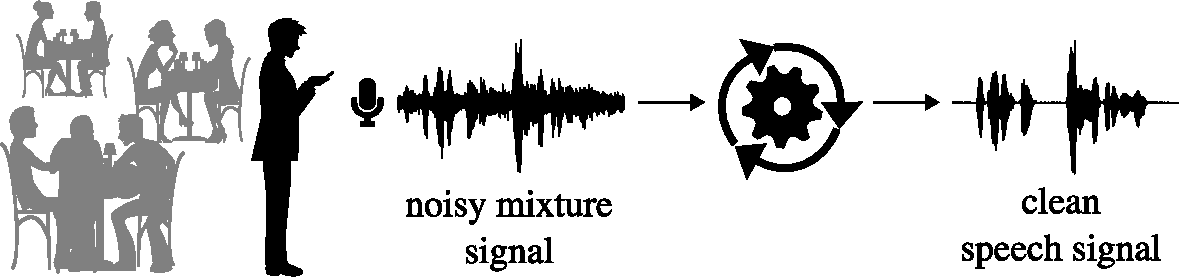
\includegraphics[scale=0.4]{images/intro_speech_enhancement.pdf}
\end{figure}
\begin{figure}
\centering
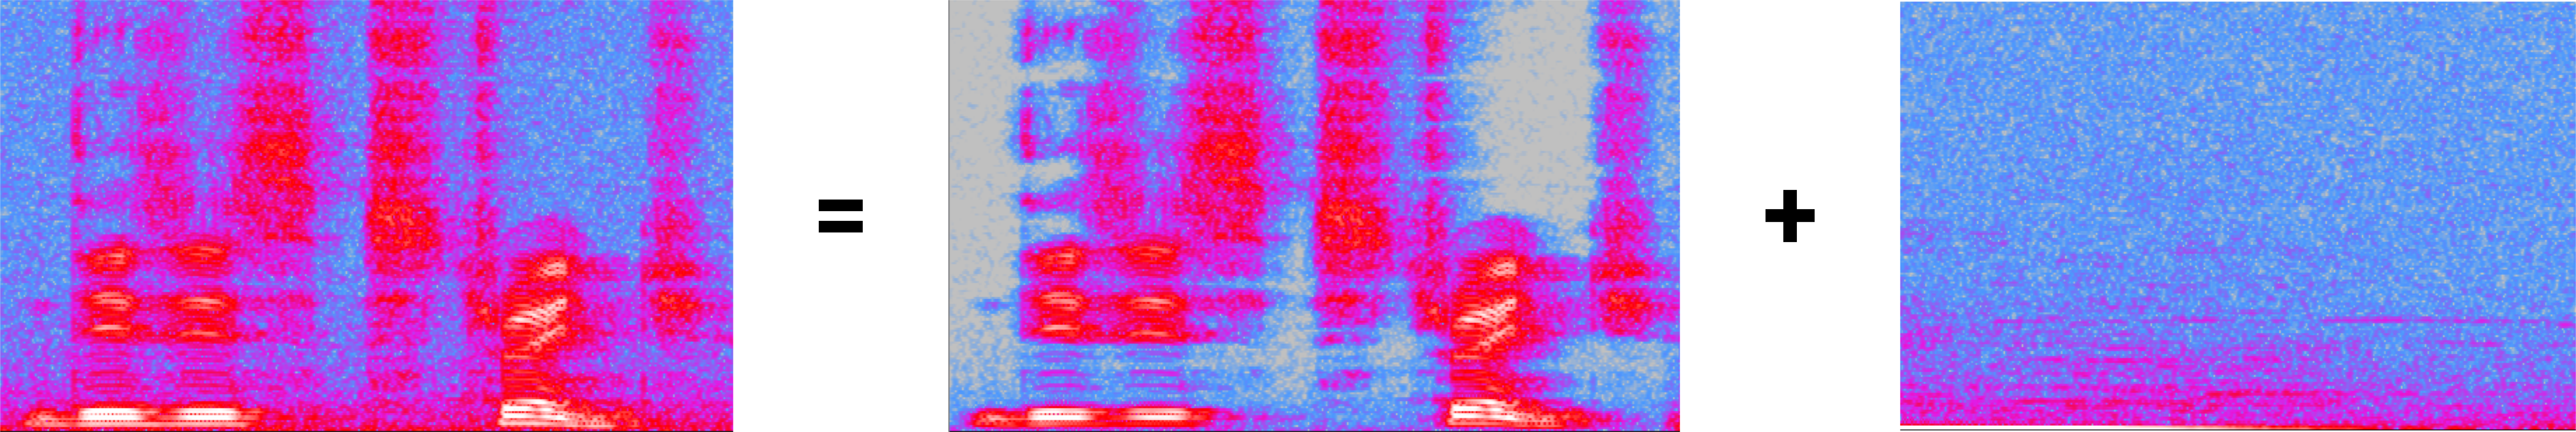
\includegraphics[width=0.8\textwidth]{images/spectrogram.png}
\end{figure}
\end{frame}

% \begin{frame}{Applications: Dereverberation}
%  \begin{figure}
%     \centering
%     \includegraphics[width=0.4\textwidth]{images/reverberation1}
%     \hspace{4mm}
%     \includegraphics[width=0.4\textwidth]{images/reverberation2}
% \end{figure}
% Remove the reflected echoes (delayed and atenuated copies of the original signal).
% \end{frame}
%
% \begin{frame}{Applications: Diarisation}
%  \begin{figure}
%   \centering
%   \includegraphics[width=0.9\textwidth]{images/diarisation}
%  \end{figure}
%
% \end{frame}

\begin{frame}{But...}
\centering
 \alert{\textbf{\Huge what about GenAI?}}
\end{frame}



\section{Visual and Audio data}

\begin{frame}{Visual data}
Cameras capture the light arriving to a planar sensor.\vspace{3mm}
 \begin{columns}
  \begin{column}{0.5\textwidth}
   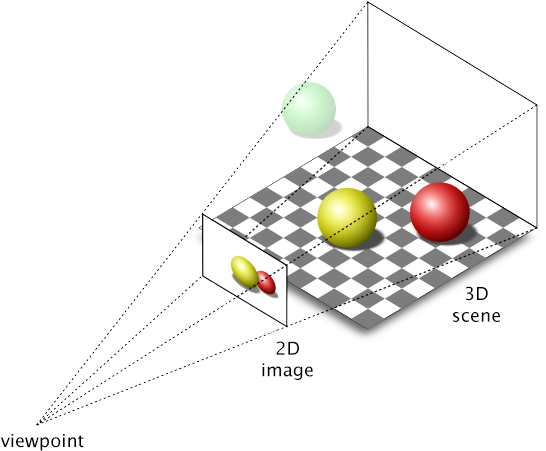
\includegraphics[width=\textwidth]{images/cameraprojection.png}  
  \end{column}
  \begin{column}{0.5\textwidth}
   \begin{itemize}
    \item Light reflects on the surfaces.
    \item The sensor counts the photons.
    \item Objects \textit{occlude} each other.\\
    (Pixels belong to one object.)
    \item Limited field of view.\\
    (Objects appear/disappear.)
   \end{itemize}
  \end{column}
 \end{columns}
\end{frame}

\begin{frame}{Auditory data}
 Microphones capture the air pressure variations.\vspace{3mm}
 \begin{columns}
  \begin{column}{0.5\textwidth}
  \centering
   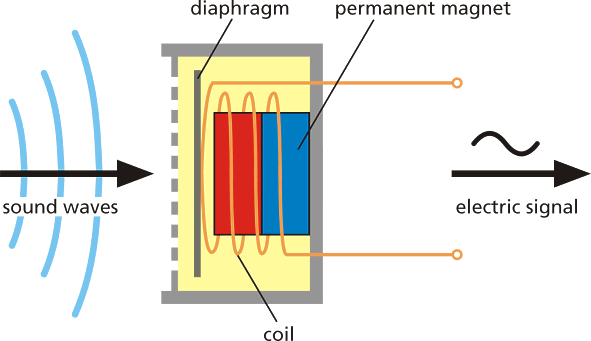
\includegraphics[width=0.8\textwidth]{images/microphone.png}  
  \end{column}
  \begin{column}{0.5\textwidth}
   \begin{itemize}
    \item Sound waves reflect on surfaces.
    \item The sensor measures air pressure variations.
    \item Objects \textit{overlap} each other.\\
    (Sound samples belong to various objects.)
    \item Quasi-omni-directional.
    \item Intermitent activity.
   \end{itemize}
  \end{column}  
 \end{columns}
\end{frame}

\begin{frame}{Audio-visual data}
 How to relate information in different modalities (audio and video)?\\
 \begin{itemize}
  \item Synchronisation
  \item Calibration
  \item Semantic correspondence
 \end{itemize}
  \begin{columns}
  \begin{column}{0.5\textwidth}
  \centering
   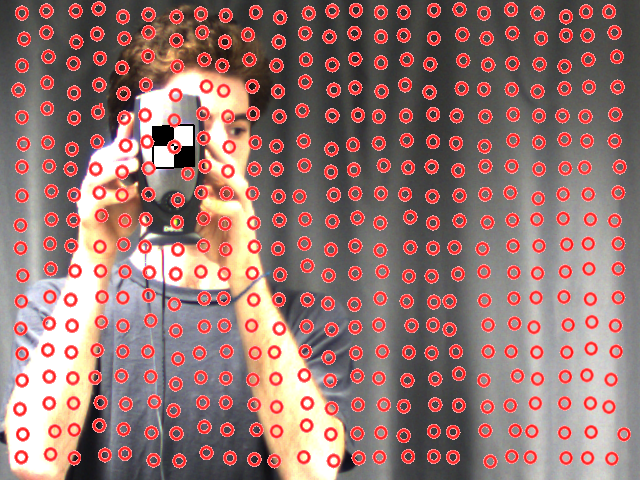
\includegraphics[width=0.65\textwidth]{images/avcalib.png}  
  \end{column}
  \begin{column}{0.5\textwidth}
  \centering
   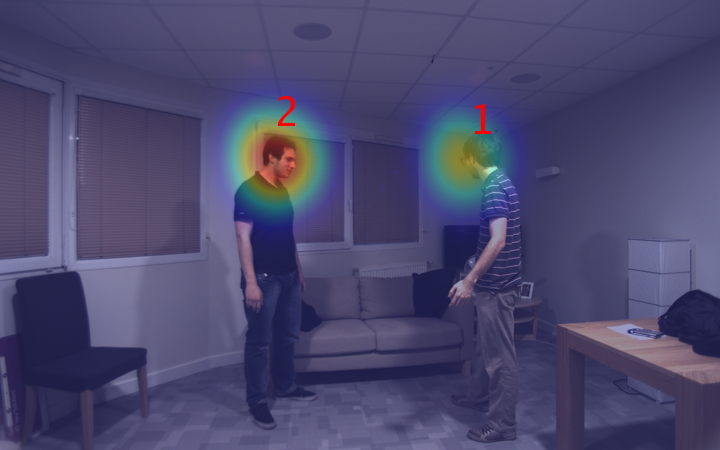
\includegraphics[width=0.8\textwidth]{images/avtracking.png}  
  \end{column}  
 \end{columns}
\end{frame}

\begin{frame}{Challenges in each modality}
 So why using various modalities? Because of their limitations.\vspace{3mm}

%  \begin{columns}
%   \begin{column}{0.8\textwidth}
 Vision:\vspace{-2mm}
 {\small\begin{itemize}
  \item Low resolution if far away.\vspace{-2mm}
  \item Blur, occlusions, variable lighting conditions.\vspace{-2mm}
  \item People/objects cropped/appearing/disappearing.\vspace{-2mm}
  \item Changes in appearance.
 \end{itemize}}

 Audio:\vspace{-2mm}
 {\small\begin{itemize}
  \item Speaker overlap.\vspace{-2mm}
  \item Background noise (and other undesired sources).\vspace{-2mm}
  \item Presence of reverberations.\vspace{-2mm}
  \item Impact of the body on which\\ the microphones are mounted.
 \end{itemize}} 
%   \end{column}
%   \begin{column}{0.2\textwidth}
%   \centering
\vspace{-4cm}
\begin{flushright}
 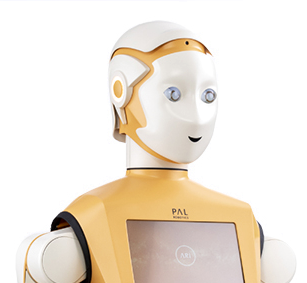
\includegraphics[width=0.35\textwidth]{images/ARIrobot.png}   
\end{flushright}
%   \end{column}  
%  \end{columns}
\end{frame}

% \begin{frame}{Objectives of MLVA}
%  \begin{enumerate}
%   \item To understand how to represent auditory and visual data.
%   \item To learn to develop machine learning models/methods to exploit auditory and visual data.
%   \item To introduce deep neural networks for audio and vision.
%   \item To understand the limitations of mono-modal machine learning.
%   \item To get a glance on how to use machine learning (specifically neural networks) for audio-visual processing.
%  \end{enumerate}\vspace{4mm}
%  {\small (Comment on adversarial (GAN) and variational (VAE) strategies)}
% \end{frame}

% 
% \section{Audio data}
% 
% \begin{frame}{The raw data}
%   Microphones capture the air pressure variations.\vspace{3mm}
%  
%   This \textit{continuous} signal is \textit{sampled} into a \textit{discrete} signal.
%   \begin{figure}
%    \centering
%    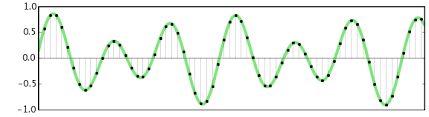
\includegraphics[width=0.7\textwidth]{images/sampling.png}
%   \end{figure}
% 
%   We never work with $x(t)$ but rather with $x[n]=x(t=nT)$.\\
%   Where $T$ is the sampling period.
% \end{frame}
% 
% \begin{frame}{The Nyquist frequency}
%  What is the problem with sampling?
%  \begin{figure}
%   \centering
%   \only<1>{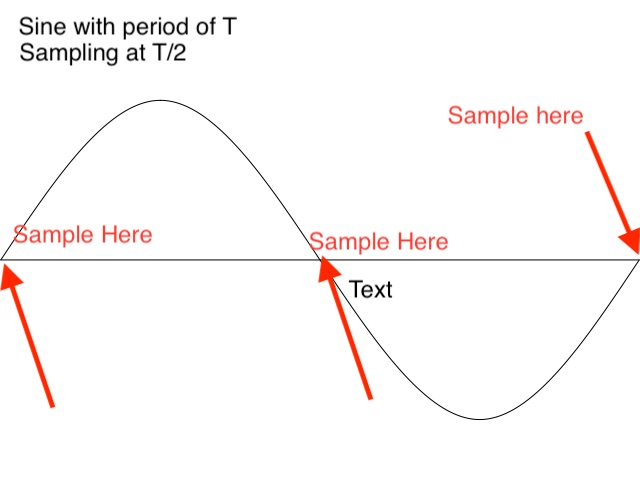
\includegraphics[width=0.5\textwidth]{images/nyquist1.jpg}}%
%   \only<2>{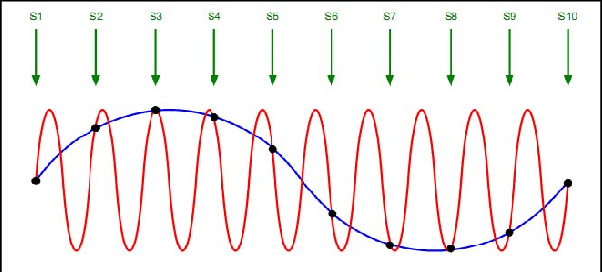
\includegraphics[width=0.5\textwidth]{images/nyquist2.png}}
%  \end{figure}
%  \begin{block}{Nyquist-Shanon Sampling Theorem}
%   If a continuous signal is sampled at a frequency $F_s$, we can only reconstruc the content corresponding to frequencies $<F_s/2$.
%  \end{block}
% \end{frame}
% 
% \begin{frame}{Every-day example of this}
% The phone!
%  \begin{itemize}
%   \item Speech signal can contain energy up to $20$~kHz.
%   \item Most of the energy is within the range $0.3$-$3$~kHz.
%   \item This is why the phone standards sample at $8$~kHz.
%   \item Keeping most of the content.
%   \item Losing high-frequency details - \textit{telephone voice} effect.
%  \end{itemize}\vspace{4mm}
% Two VERY important operations with discrete signals:
%  \begin{itemize}
%   \item convolution,
%   \item discrete Fourier transform.
%  \end{itemize}
% \end{frame}
% 
% \begin{frame}{The Convolution}
% 
%   \begin{columns}
%   \begin{column}{0.5\textwidth}
% Convolution requires two signals: the input signal $f$ and the kernel signal $k$.\vspace{3mm}
% 
% The convolution is denoted and defined as:
% \[ (f * g)[n] = \sum_m f[m] g[n-m]. \] 
%   \end{column}
%   \begin{column}{0.5\textwidth}
%   \centering
%    \includegraphics[width=0.8\textwidth]{images/convolution.png}  
%   \end{column}  
%  \end{columns}
% \end{frame}
% 
% \begin{frame}{The Convolution (II)}
%  Example: $f=[7,4,-3,6,-8]$ and $g=[1,1,-1]$.\\
%  {\footnotesize Arrays start at zero: $f[0]=7$, $g[0]=1$.}\vspace{2mm}\\
%  
%  Let's play!\\
%  $(f*g)[0]=\pause \sum_m f[m] g[-m] = 7$\\\pause
%  $(f*g)[1]=\pause \sum_m f[m] g[1-m] = 11$\\\pause
%  $(f*g)[2]=\pause \sum_m f[m] g[2-m] = -6$\\\pause
%  $(f*g)[3]=\pause \sum_m f[m] g[3-m] = -1$\\\pause
%  $(f*g)[4]=\pause \sum_m f[m] g[4-m] = 1$\\\pause
%  $(f*g)[5]=\pause \sum_m f[m] g[5-m] = -14$\\\pause
%  $(f*g)[6]=\pause \sum_m f[m] g[6-m] = 8$\vspace{3mm}\\\pause
%  
%  What is the length of the output signal? \pause $\textrm{len}((f * g)) = \textrm{len}(f) + \textrm{len}(g) - 1$.
% \end{frame}
% 
% \begin{frame}{The Convolution (III)}
%  Properties:
%  \begin{itemize}
%   \item Linear: $(f*(g+h)) = (f*g) + (f*h)$.
%   \item Associativity: $((f*g)*h) = (f*(g*h))$.
%   \item Commutativity: $(f*g)=(g*f)$.
%   \item ...
%  \end{itemize}\vspace{3mm}
% 
%  
%  Modes:
%  \begin{itemize}
%   \item \textcolor{blue}{Full} (as in the previous slide): all outputs are kept.
%   \item \textcolor{red}{Same} the output has the same length as the input.
%   \item \textcolor{green}{Valid} only outputs involving the full input/kernel signal are kept.
%  \end{itemize}
%  \[(f*g) = [\underbrace{7,\underbrace{11,\underbrace{-6,-1,1}_{\textcolor{green}{Valid}},-14}_{\textcolor{red}{Same}},8}_{\textcolor{blue}{Full}}]\]
% \end{frame}
% 
% \begin{frame}{The 2D \& 3D Convolution}
%  Higher dimensional versions of the convolution operator exist: \vspace{3mm}
%    \begin{columns}
%   \begin{column}{0.5\textwidth}
%    \centering
%    \includegraphics[width=0.8\textwidth]{images/2dconvolution.png}  
%   \end{column}
%   \begin{column}{0.5\textwidth}
%   \centering
%    \includegraphics[width=0.8\textwidth]{images/3dconvolution.png}  
%   \end{column}  
%  \end{columns}\vspace{3mm}
%  
%  In which ``mode'' are these schemes? (Full, Same, Valid)
% \end{frame}
% 
% \begin{frame}{The discrete Fourier transform}
%  Purpose: structure the information in frequencies instead of time.\vspace{2mm}\\
%  Input: signal in the time domain $f[0],\ldots,f[L-1]$.\vspace{2mm}\\
%  Output: a sequence of $L$ complex numbers describing the magnitude and phase at each frequency bin.\vspace{2mm}\\
%  Formula: \[F[k] = \sum_{n=0}^{L-1} f[n] \exp\left(-i\frac{2\pi}{L}kn\right).\]
%  Fast Fourier transform: an efficient algorithm to compute DFT when $L$ is a power of 2.
% \end{frame}
% 
% \begin{frame}{The discrete Fourier transform (II)}
%  Fourier domain decomposes the signal in frequencies not in time:\\
%  \begin{figure}
%   \centering
%   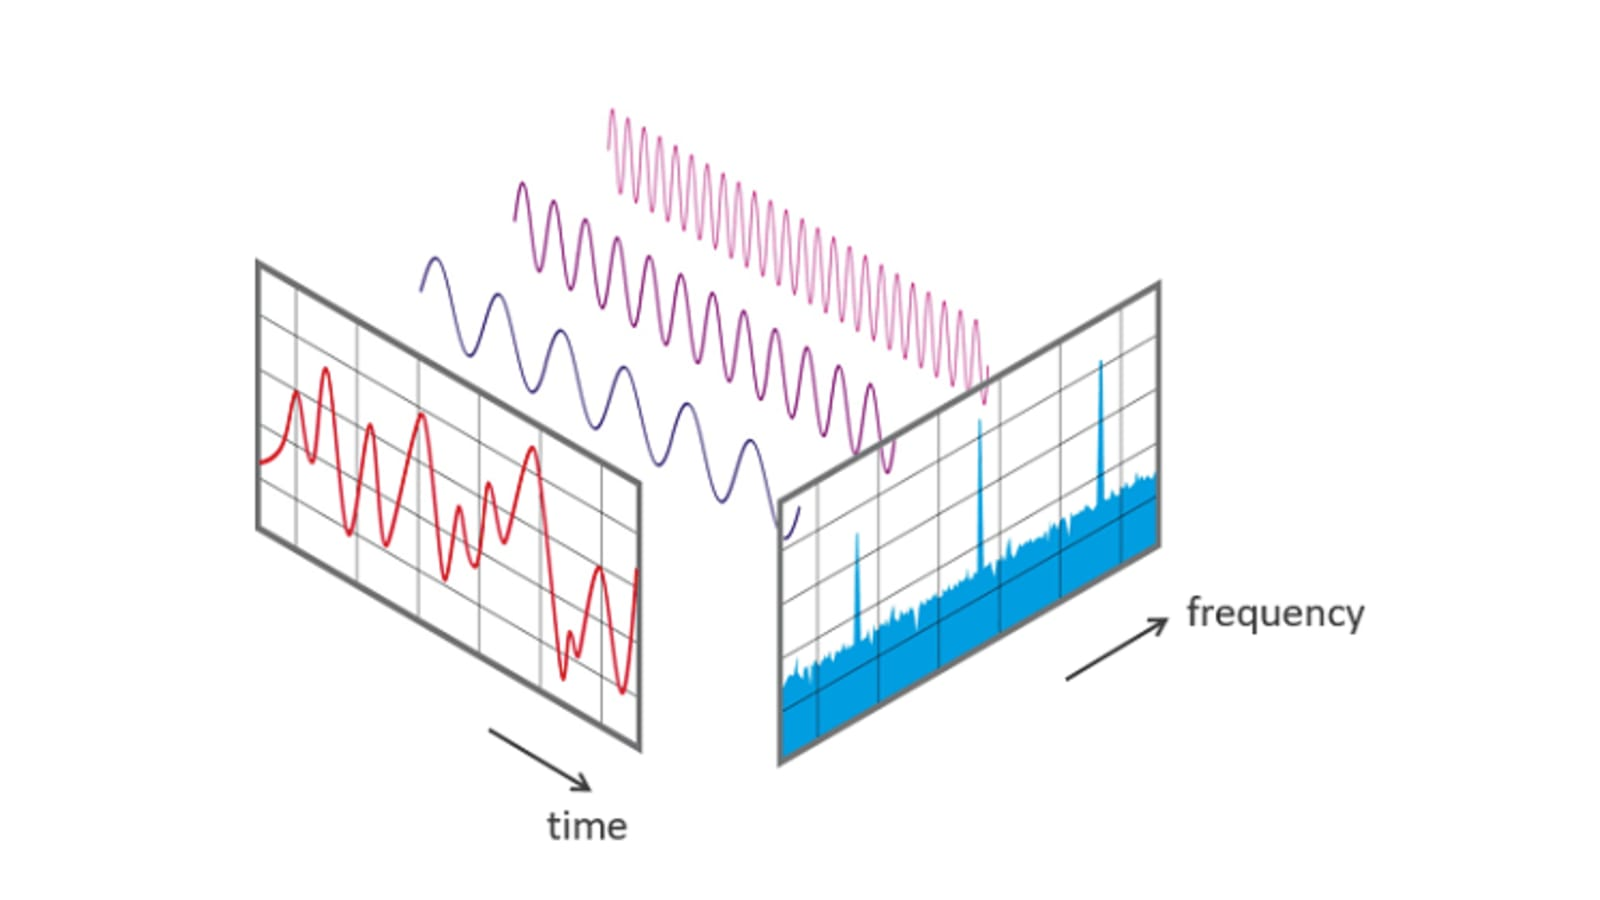
\includegraphics[width=0.8\textwidth]{images/fourierdomain.png}
%  \end{figure}
%  Problem: we have to choose either time \textit{or} frequency.
% \end{frame}
% 
% \begin{frame}{The short-time Fourier transform}
%  STFT: segment the input signal, and apply DFT to each segment.
% \begin{figure}
% \centering
% 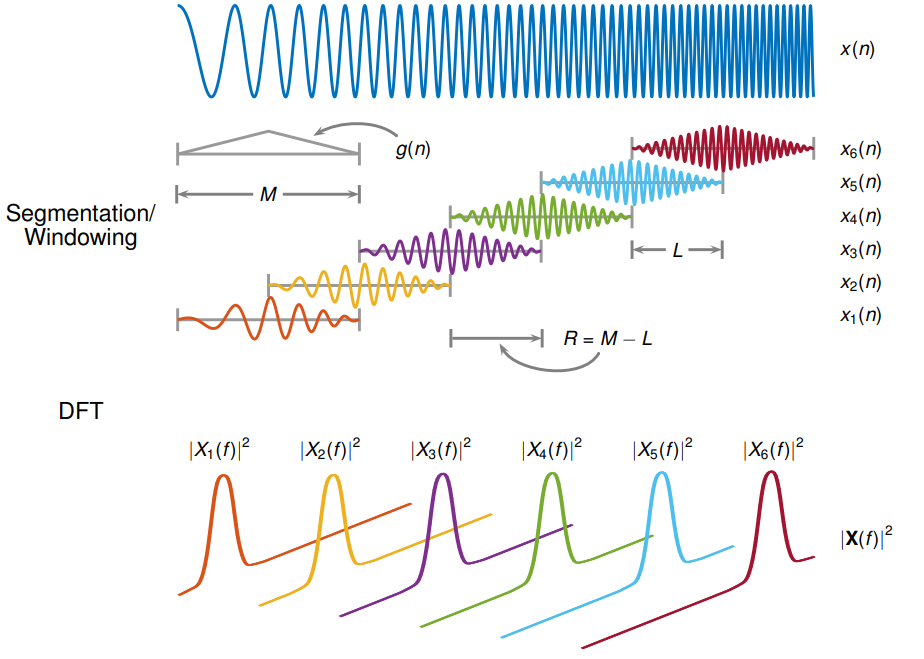
\includegraphics[width=0.75\textwidth]{images/stft.png}
% \end{figure}
% 
% \alert{Let's check that with a nice wav file!}
% \end{frame}
% 
% \begin{frame}{STFT comments}
%  \begin{itemize}
%   \item There is a duality:
%   \begin{itemize}
%    \item Represent the frequential content at a given time.
%    \item Represent the evolution of a given frequency over time.
%   \end{itemize}\vspace{3mm}
%   \item STFT requires to \textit{window} the signal with a kernel.\\
%   Different kernels lead to different properties (e.g.\ reconstruction).\vspace{3mm}
%   \item Other parameters: the window length and overlap.\\
%   They provide the rate of frequency vectors (DFT outputs).\\
%   If correctly chosen the correspond to, e.g.\ video frames.\vspace{3mm}
%  \end{itemize}
%     \centering
%     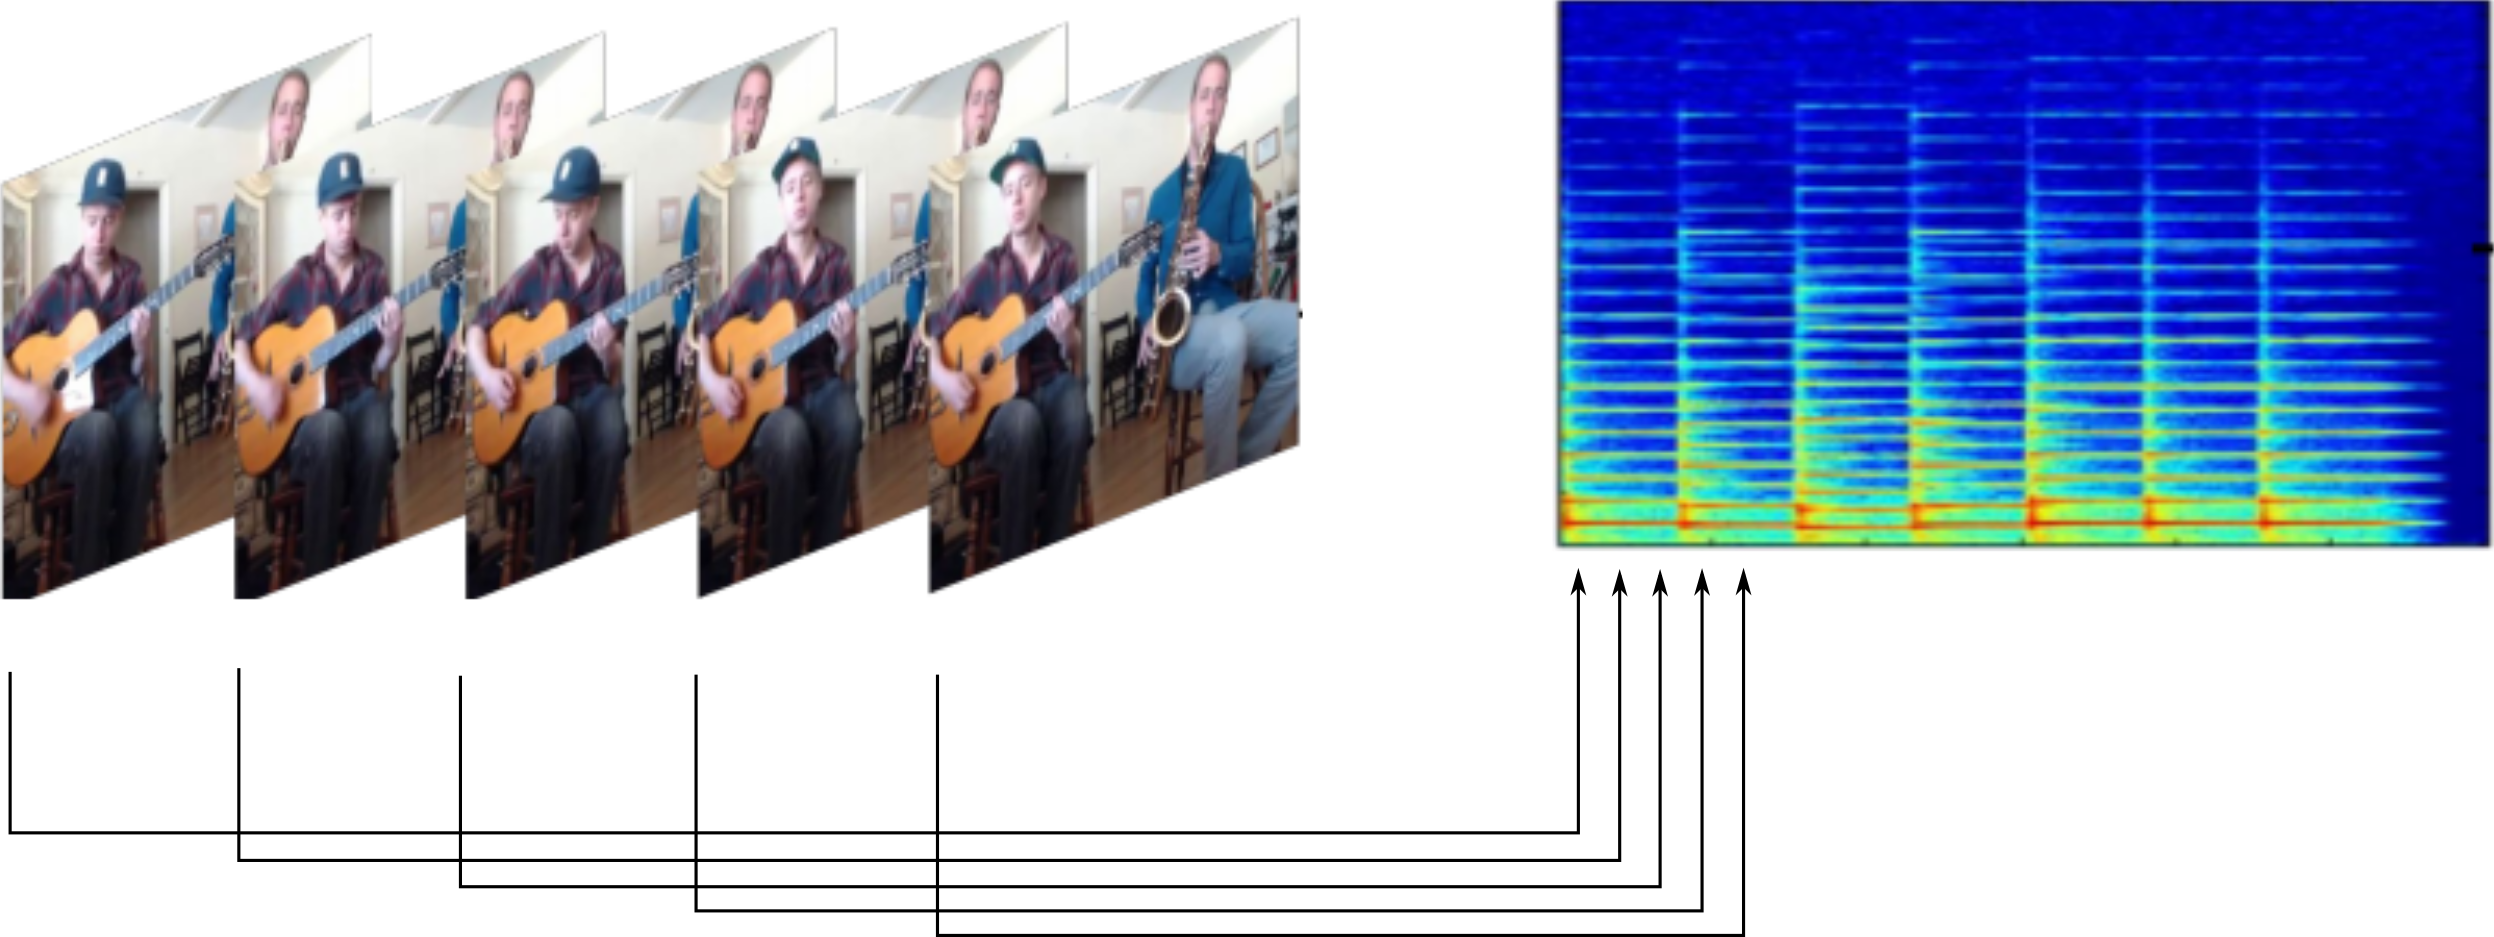
\includegraphics[width=0.6\textwidth]{images/avcorrespondence.png}
% \end{frame}


\section{Basics on Machine Learning}

\begin{frame}{Common strategy: optimisation (for machine learning)}
Optimisation is central in machine learning. As an example, supervised learning consists on estimating a {\bf prediction function} $f:{\cal X}\rightarrow{\cal Y}$ given a set of labeled training data $\{(x_n,y_n)\}_{n=1}^N$, $x_n\in{\cal X}$ and $y_n\in{\cal Y}$:
$$\min_{f\in{\cal F}} {\color{green}\underbrace{\frac{1}{N}\sum_{n=1}^N L(y_n,f(x_n))}_{\text{Empirical Risk}}} + {\color{blue} \underbrace{\lambda \Omega(f)}_{\text{Regularisation}} } $$

\pause
\begin{itemize}
 \item ${\cal X}$ is the data space and $x_n$ are the data points (visual features, bag-of-words, cepstral coefficients, raw images).\pause
 \item ${\cal Y}$ is the label space and $y_n$ are the labels (${\cal Y}$ could be $\{-1,1\}$, $\{1,\ldots,K\}$ for binary/multiclass class., $\mathbb{R}$, $\mathbb{R}^K$) for regression).\pause
 \item {\color{green} $L$ is the loss assessing the \textit{dissimilarity} between $y_n$ and $f(x_n)$.}\pause
 \item {\color{blue} $\Omega$ is the regulariser, ensuring that the optimal $f$ is \textit{reasonable}.}
\end{itemize}
\end{frame}

% \begin{frame}{Examples}
%  Examples of linear models on a $P$-dimensional feature space:
%  \begin{itemize}
%   \item Linear SVM: $ \displaystyle\min_{w\in\mathbb{R}^P} \frac{1}{N} \sum_{n=1}^N {\color{green}\max(0,1-y_n w^\top x_n)} + \lambda\|w\|^2_2. $
%   \item Ridge: $ \displaystyle\min_{w\in\mathbb{R}^P} \frac{1}{N} \sum_{n=1}^N {\color{red}\frac{1}{2}(y_n - w^\top x_n)^2} + \lambda\|w\|^2_2. $
%   \item Logistic: $ \displaystyle\min_{w\in\mathbb{R}^P} \frac{1}{N} \sum_{n=1}^N {\color{blue}\log(1+e^{(-y_n w^\top x_n)})} + \lambda\|w\|^2_2. $
%  \end{itemize}
%  
%  \centering
%  \includegraphics[width=0.7\textwidth]{images/losses.png}
% 
% \end{frame}

\begin{frame}{Overall strategy}
 The previous formulation is called \textit{empirical risk minimisation}:
 \begin{itemize}
  \item<1-> \textbf{Observe} the world, i.e.\ gather (and annotate) data.
  \item<2-> \textbf{Model} the observed data. {\color{green}Design, learn} and {\color{blue}select} the model.
  \item<3-> \textbf{Assess} the quality of the model on {\bf\color{red} test} data.
 \end{itemize}
 \centering
 \only<1>{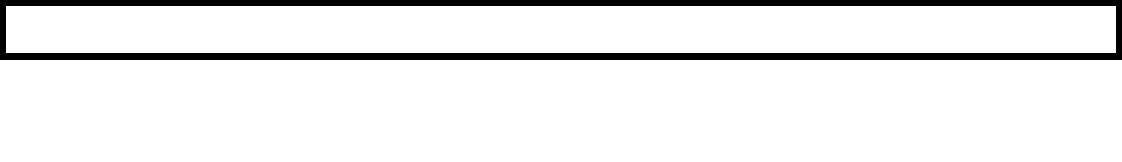
\includegraphics[width=0.9\textwidth]{images/trainingsplit-pre.pdf}}%
 \only<2>{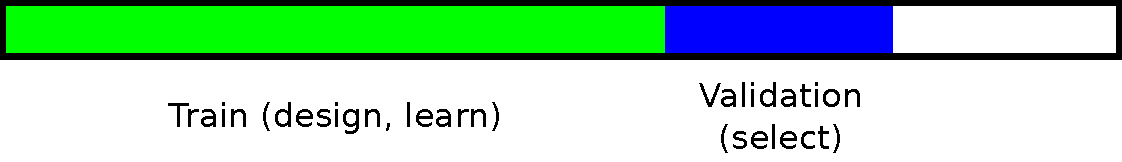
\includegraphics[width=0.9\textwidth]{images/trainingsplit-notest.pdf}}%
 \only<3->{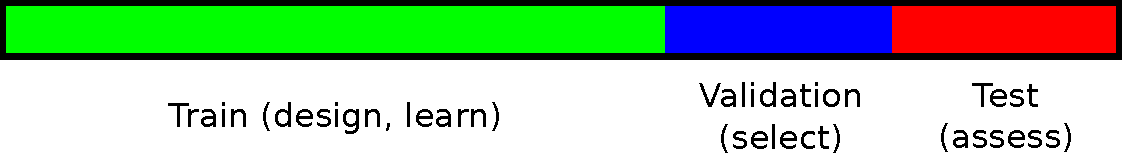
\includegraphics[width=0.9\textwidth]{images/trainingsplit.pdf}}%
 
 \only<4->{
 Test on NEW data is very important to quantify the generalisation error!!!
 \begin{block}{General principle}
  This principle is valid (and required) for a wide variety of tasks, and methods, namely: neural networks, kernel methods, etc.
 \end{block}}
\end{frame}
 
% \begin{frame}{Overall strategy: comments}
%  \begin{block}{Not so simple}
%     Even linear models lead to challenging problems in optimization: 
%     \begin{itemize}
%     \item algorithms that scale both in the problem size $N$ and dimension $P$;
%     \item are able to exploit the problem structure;
%     \item come with statistical, convergence and numerical stability guarantees.
%     \end{itemize}
%  \end{block}
%  \pause
%  \begin{block}{Usable beyond supervised learning}
%    $$\min_{f\in{\cal F}} {\color{green} \frac{1}{N}\sum_{n=1}^N L(f(x_n)) } + {\color{blue} \lambda \Omega(f) } $$
%  \begin{itemize}
%   \item $L$ is not a classification loss;
%   \item Example of paradigms: K-means, PCA, MoG, matrix factorisation.
%  \end{itemize}
%  \end{block}
% \end{frame}

%%%%%%%%%%%%%%%%%%%%%%%%%%%%%%%%%%%%%%%%%%%%%%%%%%%%%%%%%%%%%%
%%%%%%%%%%%%%%%%%%%%%%%%%%%%%%%%%%%%%%%%%%%%%%%%%%%%%%%%%%%%%%
\section{Deep Learning \textit{Basics}}

%%%%%%%%%%%%%%%%%%%%%%%%%%%%%%%%%%%%%%%%%%%%%%%%%%%%%%%%%%%%%%
\begin{frame}{What is Deep Learning?}
Deep Learning is a field of machine learning, aiming to \textbf{learn representations} of data tailored to the problem at hand.\vspace{3mm}

The conception of the model depends on the task to be solved, but the philosophy of deep learning is to process \textbf{\textit{raw} data} (e.g.\ images, sounds).\vspace{3mm}

It can be used in supervised, unsupervised and reinforcement learning. Supervised $\leftrightarrow$ annotated labels, unsupervised $\leftrightarrow$ no annotated labels, reinforcement $\leftrightarrow$ learning a sequence of actions to maximise a reward.\vspace{3mm}

Why is it called Deep Learning and Deep Neural Networks?

\end{frame}

%%%%%%%%%%%%%%%%%%%%%%%%%%%%%%%%%%%%%%%%%%%%%%%%%%%%%%%%%%%%%%
\begin{frame}{Deep Learning and Deep Neural Networks}
 \begin{block}{Neural}
   As we will see later, the basic unit is called (artificial) neuron, and its design is inspired by the way brain cells function. Several inputs (scalars) are weighted and added, to trigger (or not) the single output (scalar).\\
 \end{block}
%  \pause
 \begin{block}{Deep Network}
   These neurons are grouped in layers, in different structures. To construct a network, we stack $K$ layers on top of each other.\vspace{3mm}\\
   Weighted sum $\leftrightarrow$ linear operator ($A$), trigger $\leftrightarrow$ non-linear function ($\sigma$).\vspace{-3mm}
   $$ f(x) = \sigma_K(A_K \sigma_{K-1}( A_{K-1} \cdots \sigma_2(A_2\sigma_1(A_1x))\cdots)). $$
 \end{block}
%  \pause
 \begin{block}{Learning}
  Once we have decided the structure, we need to devise a way to optimise for the parameters of the linear operators: $A_1,\ldots,A_K$.
 \end{block}
\end{frame}

%%%%%%%%%%%%%%%%%%%%%%%%%%%%%%%%%%%%%%%%%%%%%%%%%%%%%%%%%%%%%%
\begin{frame}{How to learn?}
 \begin{columns}
  \begin{column}{0.5\textwidth}
  \centering
   
\includegraphics[width=0.85\textwidth]{figs/I/deeplearningprocess.png}
  \end{column}
  \begin{column}{0.45\textwidth}
    \begin{enumerate}
     \item Sample a batch of annotated data.
     \item Forward the network to predict, $f(x)$.
     \item Compute the prediction error for back-propagation.
     \item Update the weights by back-propagation.
    \end{enumerate}
  \end{column}
 \end{columns}\vspace{3mm}
 We first generate an \textbf{error signal} measuring the difference between predictions and ground-truth (annotations). This signal is used to \textbf{update the weights} of the network.
\end{frame}


%%%%%%%%%%%%%%%%%%%%%%%%%%%%%%%%%%%%%%%%%%%%%%%%%%%%%%%%%%%%%%
\begin{frame}{History of Deep Learning}

The history of deep learning started as early as 1950's (!).\vspace{5mm}\\

As for any successful scientific field it is controversial:\\ who did what, when, with what impact?.\vspace{5mm}

In 2018, three top scientists received the ACM \alert{\href{https://awards.acm.org/about/2018-turing
}{A. M. Turing award}}:\\ Yann LeCun, Geoffrey Hinton and Yoshua Bengio.

\end{frame}

%%%%%%%%%%%%%%%%%%%%%%%%%%%%%%%%%%%%%%%%%%%%%%%%%%%%%%%%%%%%%%
\begin{frame}{Biological motivation}
 \begin{itemize}
  \item The neuron is the basic computational unit of the brain\\
  About $10^{11}$ neurons in the human brain.\vspace{2mm}
  \item Simplified neuron model as a linear threshold unit.
  \begin{itemize}
  \item Firing rate of electrical spikes modeled as continuous output quantity
  \item Connection strength modeled by multiplicative weights
  \item Cell activation given by sum of inputs
  \item Output is non-linear function of activation
  \end{itemize}
  \item Basic component in neural circuits for complex tasks
 \end{itemize}
 \begin{center}
  
\includegraphics[width=0.5\textwidth]{figs/I/neuron.png}
  
\includegraphics[width=0.4\textwidth]{figs/I/neuron_model.jpeg}
 \end{center}\vspace{-3mm}
 \begin{flushright}
  {\tiny Figure from \url{http://cs231n.github.io/neural-networks-1/}.}
 \end{flushright}
\end{frame}

%%%%%%%%%%%%%%%%%%%%%%%%%%%%%%%%%%%%%%%%%%%%%%%%%%%%%%%%%%%%%%
\begin{frame}{Multi-Layer Perceptron (MLP)}
 \begin{itemize}
  \item Instead of using generlised linear functions, learn the features!
  \item Each unit (neuron) in MLP computes:
  \begin{enumerate}
   \item Linear function of the features (activations) in the previous layer
   \item Followed by scalar non-linearity (not the perceptron's ``step'')
  \end{enumerate}
 \end{itemize}
 \begin{columns}
  \begin{column}{0.5\textwidth}
   \only<1>{$$z_j = h^{(1)}\left(\sum_i w^{(1)}_{ij}x_i\right)$$\\
   $$y_k = h^{(2)}\left(\sum_j w^{(2)}_{jk}z_j\right)$$}
   \only<2>{\begin{itemize}
    \item If activations are linear, then it remans a linear model.
    \item Two-layer MLPs can uniformly approximate any continuous function on a
compact input domain provided a sufficiently large number of hidden units.
   \end{itemize}}
  \end{column}
  \begin{column}{0.4\textwidth}
   
\includegraphics[width=\textwidth]{figs/I/mlp.png}
  \end{column}
 \end{columns}
\end{frame}

%%%%%%%%%%%%%%%%%%%%%%%%%%%%%%%%%%%%%%%%%%%%%%%%%%%%%%%%%%%%%%
\section{Feed Forward Networks}
%%%%%%%%%%%%%%%%%%%%%%%%%%%%%%%%%%%%%%%%%%%%%%%%%%%%%%%%%%%%%%

%%%%%%%%%%%%%%%%%%%%%%%%%%%%%%%%%%%%%%%%%%%%%%%%%%%%%%%%%%%%%%
\begin{frame}{Feed Forward Networks}
 \begin{itemize}
  \item MLP Architecture can be generalized (more layers, skip-connections, etc).
  \item Feed-forward nets are restricted to directed acyclic graphs: ensures that output can be computed from the input in a single feed-forward pass.
  \begin{center}
   
\includegraphics[width=0.6\textwidth]{figs/I/feedforward.png}
  \end{center}
  \item Important issues in practice
  \begin{itemize}
   \item Designing network architecture (\# nodes, layers, non-linearities, etc)
   \item Learning the network parameters (Non-convex optimization)
   \item Sufficient training data (Data augmentation, synthesis)
  \end{itemize}
 \end{itemize}
\end{frame}

%%%%%%%%%%%%%%%%%%%%%%%%%%%%%%%%%%%%%%%%%%%%%%%%%%%%%%%%%%%%%%
\begin{frame}{Simple output case: multiclass classification}
 \begin{itemize}
  \item Each output neuron is mapped to the posterior prob. of the class:
   $$y_k \rightarrow p(c_k|x) = \frac{\exp(y_k)}{\sum_m \exp(y_m)} \quad \text{So-called \textit{softmax} operation}.$$
  \item Multi-class logistic regression loss (also called cross-entropy loss):
   $$ {\cal L} = - \sum_k t_k\log p(c_k|x) \rightarrow t_k = 1 \Leftrightarrow k \text{ is the correct class}.$$
   $\Rightarrow$ We are maximising the log-probability of the correct class.
  \item We are now learning the classifier and the data representation simultaneously $\rightarrow$ \textbf{representation learning}.\\\vspace{3mm}
  \alert{But how do we do that?}
 \end{itemize}
\end{frame}

%%%%%%%%%%%%%%%%%%%%%%%%%%%%%%%%%%%%%%%%%%%%%%%%%%%%%%%%%%%%%%
\begin{frame}{Computing the gradient}
Recall:
  \begin{columns}
  \begin{column}{0.55\textwidth}
   {\small $$ z_m = h\left(\sum_{d=0}^D w^{(1)}_{md}x_d\right),\quad y_k = h\left(\sum_{m=0}^M w^{(2)}_{km}z_m\right),$$}
   {\small $$ p(c_k|x) = \frac{e^{y_k}}{\sum_n e^{y_n}}, \quad h(u) = 1/(1+e^{-u}),$$}
   {\small $$ {\cal L} = - \sum_k t_k\log p(c_k|x), \quad t_k = 1 \text{ or } 0.$$}
  \end{column}
  \begin{column}{0.35\textwidth}
   
\includegraphics[width=\textwidth]{figs/I/mlp.png}
  \end{column}
 \end{columns}\vspace{3mm}
 Apply the chain-rule successively to ``back-propagate'' the error through the network\\ (check example in Chamilo).
\end{frame}

%%%%%%%%%%%%%%%%%%%%%%%%%%%%%%%%%%%%%%%%%%%%%%%%%%%%%%%%%%%%%%
\begin{frame}{Activation functions}
% Many possible. Simple non-linear scala functions.\vspace{4mm}
  \begin{columns}
  \begin{column}{0.55\textwidth}
   \textbf{Sigmoid}: $ h(t) = 1/(1+e^{-t}).$
   \begin{itemize}
    \item Squeezes reals to $[0,1]$.
    \item Smooth step function.
    \item Historically popular because of biologically inspired.
   \end{itemize}
  \end{column}
  \begin{column}{0.3\textwidth}
   
\includegraphics[width=\textwidth]{figs/I/sigmoid-crop.pdf}
  \end{column}
 \end{columns}

 \begin{columns}
  \begin{column}{0.55\textwidth}
   \textbf{Tan-h}: $ h(t) = (e^t-e^{-t})/(e^t+e^{-t}).$
   \begin{itemize}
    \item Squeezes reals to $[-1,1]$.
    \item Similar to sigmoid.
    \item Limitation: saturated neurons ``kill'' the gradients.
   \end{itemize}
  \end{column}
  \begin{column}{0.3\textwidth}
   
\includegraphics[width=\textwidth]{figs/I/hyperbolictangent-crop.pdf}
  \end{column}
 \end{columns}
\end{frame}

%%%%%%%%%%%%%%%%%%%%%%%%%%%%%%%%%%%%%%%%%%%%%%%%%%%%%%%%%%%%%%
\begin{frame}{Activation functions}
  \begin{columns}
  \begin{column}{0.55\textwidth}
   \textbf{ReLU}: $ h(t) = \max(0,t).$
   \begin{itemize}
    \item Rectified Linear Unit.
    \item Does not saturate.
    \item Converges much faster than previous. Widely used.
   \end{itemize}
  \end{column}
  \begin{column}{0.3\textwidth}
   
\includegraphics[width=\textwidth]{figs/I/relu-crop.pdf}
  \end{column}
 \end{columns}

 \begin{columns}
  \begin{column}{0.55\textwidth}
   \textbf{Leaky ReLU}: $ h(t) = \max(\alpha t,t).$
   \begin{itemize}
    \item Does not saturate in neither region.
    \item Computationally efficient.
    \item Faster convergence.
   \end{itemize}
  \end{column}
  \begin{column}{0.3\textwidth}
   
\includegraphics[width=\textwidth]{figs/I/leakyrelu-crop.pdf}
  \end{column}
 \end{columns}
\end{frame}

%%%%%%%%%%%%%%%%%%%%%%%%%%%%%%%%%%%%%%%%%%%%%%%%%%%%%%%%%%%%%%
\begin{frame}{Training feedforward neural networks}
 \begin{itemize}
  \item Non-convex optimisation problem in very high dimension (millions!).
  $$ \frac{1}{N} \sum_{n=1}^N {\cal L}(\phi(x;W),l) + \lambda\Omega(W), \quad \phi(\cdot;W) \text{ is the DNN}.$$
  \item Many equivalent local minima exist.
  \item Regularisation, $\Omega$: using ``weight decay'' or ``drop-out.''
  \item Label smoothing to avoid overfitting: $${\cal L} = (1-\epsilon)\log(p(l|x)) + \epsilon\log(1-p(l|x)).$$
  \item Weight update using gradient descent. For large datasets, we will use batch-stochastic techniques.
 \end{itemize}
\end{frame}

%%%%%%%%%%%%%%%%%%%%%%%%%%%%%%%%%%%%%%%%%%%%%%%%%%%%%%%%%%%%%%
\begin{frame}{Training feedforward neural networks (II)}
 \begin{center}
  
\includegraphics[width=0.3\textwidth]{figs/I/deeplearningprocess.png}\hspace{3mm}
  
\includegraphics[width=0.6\textwidth]{figs/I/feedforward.png}
 \end{center}
  \begin{enumerate}
   \item Sample a batch of data (input-output) from the dataset.
   \item Feed-forward the data through the network.
   \item Back-propagate the error through the network (gradient chain rule).
   \item Update the weights with gradient.
  \end{enumerate}
\end{frame}

%%%%%%%%%%%%%%%%%%%%%%%%%%%%%%%%%%%%%%%%%%%%%%%%%%%%%%%%%%%%%%
\section{Fundamentals of ConvNets}
%%%%%%%%%%%%%%%%%%%%%%%%%%%%%%%%%%%%%%%%%%%%%%%%%%%%%%%%%%%%%%

%%%%%%%%%%%%%%%%%%%%%%%%%%%%%%%%%%%%%%%%%%%%%%%%%%%%%%%%%%%%%%
\begin{frame}{Motivation}
 \begin{center}
  
\includegraphics[width=0.5\textwidth]{figs/I/deepfeedforward.png}
 \end{center}
Is this input representation suitable for images?
\begin{center}
 
\includegraphics[height=2cm]{figs/I/airplane1.jpg}
 
\includegraphics[height=2cm]{figs/I/dog.jpg}
 
\includegraphics[height=2cm]{figs/I/table.jpg}
 
\includegraphics[height=2cm]{figs/I/cat.jpg}
\end{center}

\end{frame}

%%%%%%%%%%%%%%%%%%%%%%%%%%%%%%%%%%%%%%%%%%%%%%%%%%%%%%%%%%%%%%
\begin{frame}{CNN: Overview}
\begin{itemize}
 \item A convolutional neural network is a special feedforward network
 \item Hidden units are organized into grid, as is the input
 \item Linear mapping from layer to layer takes form of convolution
 \begin{itemize}
    \item Translation invariant processing
    \item Local processing
    \item Decouples \# of parameters from input size
    \item Same net can process inputs of varying size
 \end{itemize}
\end{itemize}
\begin{center}
 
\includegraphics[width=0.9\textwidth]{figs/I/aCNN.png}
\end{center}

\end{frame}

%%%%%%%%%%%%%%%%%%%%%%%%%%%%%%%%%%%%%%%%%%%%%%%%%%%%%%%%%%%%%%
\begin{frame}{2D convolutions}
2D convolutions are linear operations:
\begin{center}
 
\includegraphics[width=0.8\textwidth]{figs/I/2d_convolution_pa3.png}
\end{center}
\begin{itemize}
 \item Start from the top-left position.
 \item Multiply-and-add.
 \item Store in the output image.
 \item Go to next pixel position.
\end{itemize}
There are many different types of convolutions: \url{http://deeplearning.net/software/theano/tutorial/conv_arithmetic.html}.
\end{frame}

%%%%%%%%%%%%%%%%%%%%%%%%%%%%%%%%%%%%%%%%%%%%%%%%%%%%%%%%%%%%%%
\begin{frame}{Convolutions in ConvNets}
In ConvNets (or CNNs), the convolution filters or kernels have {\color{blue}depth}:
\begin{center}
 
\includegraphics[width=0.7\textwidth]{figs/I/cnn1.png}
\end{center}
\begin{flushright}
 {\footnotesize Slide from: Fei-Fei Li \& Andrej Karpathy \& Justin Johnson}
\end{flushright}
\end{frame}

%%%%%%%%%%%%%%%%%%%%%%%%%%%%%%%%%%%%%%%%%%%%%%%%%%%%%%%%%%%%%%
\begin{frame}{Convolutions in ConvNets (II)}
What is the width and height of the output image?
 \begin{center}
 
\includegraphics[width=0.7\textwidth]{figs/I/cnn2.png}
\end{center}
\begin{flushright}
 {\footnotesize Slide from: Fei-Fei Li \& Andrej Karpathy \& Justin Johnson}
\end{flushright}
\end{frame}

%%%%%%%%%%%%%%%%%%%%%%%%%%%%%%%%%%%%%%%%%%%%%%%%%%%%%%%%%%%%%%
\begin{frame}{Convolutions in ConvNets (III)}
 \begin{center}
 
\includegraphics[width=0.7\textwidth]{figs/I/cnn3.png}
\end{center}
\begin{flushright}
 {\footnotesize Slide from: Fei-Fei Li \& Andrej Karpathy \& Justin Johnson}
\end{flushright}
\end{frame}

%%%%%%%%%%%%%%%%%%%%%%%%%%%%%%%%%%%%%%%%%%%%%%%%%%%%%%%%%%%%%%
\begin{frame}{Convolutions in ConvNets (IV)}
 \begin{center}
 
\includegraphics[width=0.7\textwidth]{figs/I/cnn4.png}
\end{center}
\begin{flushright}
 {\footnotesize Slide from: Fei-Fei Li \& Andrej Karpathy \& Justin Johnson}
\end{flushright}
\end{frame}

%%%%%%%%%%%%%%%%%%%%%%%%%%%%%%%%%%%%%%%%%%%%%%%%%%%%%%%%%%%%%%
\begin{frame}{Convolutions in ConvNets (V)}
 \begin{center}
 
\includegraphics[width=0.7\textwidth]{figs/I/cnn5.png}
\end{center}
\begin{flushright}
 {\footnotesize Slide from: Fei-Fei Li \& Andrej Karpathy \& Justin Johnson}
\end{flushright}
\end{frame}

%%%%%%%%%%%%%%%%%%%%%%%%%%%%%%%%%%%%%%%%%%%%%%%%%%%%%%%%%%%%%%
\begin{frame}{Convolutions in ConvNets (VI)}
The filters \textbf{must} have the same depth as the input. The output depth corresponds to the number of filters.
 \begin{center}
 
\includegraphics[width=0.4\textwidth]{figs/I/cnn6.png}
\end{center}
\begin{flushright}
 {\footnotesize Slide from: Fei-Fei Li \& Andrej Karpathy \& Justin Johnson}
\end{flushright}
\end{frame}

%%%%%%%%%%%%%%%%%%%%%%%%%%%%%%%%%%%%%%%%%%%%%%%%%%%%%%%%%%%%%%
\begin{frame}{Convolutions in ConvNets (VII)}
We can repeat the operation with a second convolutional layer.
 \begin{center}
 
\includegraphics[width=0.8\textwidth]{figs/I/cnn-end.png}
\end{center}
\begin{flushright}
 {\footnotesize Slide from: Fei-Fei Li \& Andrej Karpathy \& Justin Johnson}
\end{flushright}
\end{frame}

%%%%%%%%%%%%%%%%%%%%%%%%%%%%%%%%%%%%%%%%%%%%%%%%%%%%%%%%%%%%%%
\begin{frame}{Pooling}
 \begin{itemize}
  \item Applied separately per feature channel
  \item Effect: invariance to small translations of the input
  \item Max and average pooling most common, other things possible
  \item Parameter free layer
  \item Similar to strided convolution with special non-trainable filter
 \end{itemize}
   \begin{center}
 
\includegraphics[width=0.4\textwidth]{figs/I/pooling.png}
\end{center}
\end{frame}

%%%%%%%%%%%%%%%%%%%%%%%%%%%%%%%%%%%%%%%%%%%%%%%%%%%%%%%%%%%%%%
\begin{frame}{Receptive field}
 \begin{itemize}
  \item Receptive field” is area in original image impacting a certain unit.\\
  Later layers can capture more complex patterns over larger areas.
  \item Receptive field size grows linearly over convolutional layers.\\
  If we use a convolutional filter of size $w\times w$, then each layer the receptive
  field increases by $w-1$.
 \end{itemize}
   \begin{center}
 
\includegraphics[width=0.4\textwidth]{figs/I/receptivefield.png}
\end{center}
\end{frame}

%%%%%%%%%%%%%%%%%%%%%%%%%%%%%%%%%%%%%%%%%%%%%%%%%%%%%%%%%%%%%%
\begin{frame}{Fully connected layers}
\begin{itemize}
 \item Convolutional and pooling layers typically followed by several ``fully
connected'' (FC) layers, i.e. a standard MLP
 \item FC layer connects all units in previous layer to all units in next layer
 \item Assembles all local information into global vectorial representation
\begin{center}
 
\includegraphics[width=0.9\textwidth]{figs/I/smallcnn.png}
\end{center}
\end{itemize}
\end{frame}

%%%%%%%%%%%%%%%%%%%%%%%%%%%%%%%%%%%%%%%%%%%%%%%%%%%%%%%%%%%%%%
\begin{frame}{Drop-out regularisation}
 \begin{itemize}
  \item Main idea: deactivate a subset of neurons, randomly selected at every batch during training.
  \item If forces the network to be redundant, hence robust.
  \item Different paths to recognise the same pattern.
 \end{itemize}
\begin{center}
 
\includegraphics[width=0.9\textwidth]{figs/I/dropout.png}
\end{center}
\end{frame}

%%%%%%%%%%%%%%%%%%%%%%%%%%%%%%%%%%%%%%%%%%%%%%%%%%%%%%%%%%%%%%
\begin{frame}{Batch normalisation}
 \begin{itemize}
  \item Motivation: for very deep networks with ReLU, we quickly overflow (very large values).
  \item Main idea: the output of the linear combinations must follow a standard Gaussian distribution (zero mean, unit variance).
  \item Rationale: then all layers work at a similar regime.
  \item Usually after the fully connected or convolutional layers and before the non-linear activation.
  \item Compute the mean and variance for each neuron and:
  $$x^{\textrm{new}} = \frac{x^{\textrm{old}}-\mu}{\sqrt{\nu}}$$.
  \item Improves gradient flow and allows for larger learning rates.
  \item It is an unsupervised process that can take place at test time as well.
 \end{itemize}
\end{frame}

%%%%%%%%%%%%%%%%%%%%%%%%%%%%%%%%%%%%%%%%%%%%%%%%%%%%%%%%%%%%%%
\section{CNN Architectures}
%%%%%%%%%%%%%%%%%%%%%%%%%%%%%%%%%%%%%%%%%%%%%%%%%%%%%%%%%%%%%%

%%%%%%%%%%%%%%%%%%%%%%%%%%%%%%%%%%%%%%%%%%%%%%%%%%%%%%%%%%%%%%
\begin{frame}{AlexNet CNN (2012)}
 \begin{itemize}
  \item Winner ImageNet 2012 image classification challenge, huge impact (+50k citations). CNNs improving ``traditional'' computer vision techniques.
  \item Compared to LeNet
  \begin{itemize}
    \item Inputs at 224x224 rather than 32x32
    \item 5 rather than 3 conv layers (more feature channels in each layer)
    \item $\sim60$ million parameters
    \item ReLU non-linearity
 \end{itemize}
 \end{itemize}
\begin{center}
 
\includegraphics[width=0.7\textwidth]{figs/I/alexnet.png}
\end{center}
\end{frame}

%%%%%%%%%%%%%%%%%%%%%%%%%%%%%%%%%%%%%%%%%%%%%%%%%%%%%%%%%%%%%%
\begin{frame}{VGG CNN (2015)}
 \begin{itemize}
  \item Double the number of layers (up to 16/19).
  \item Only small $3\times3$ filters (rather than 11 in AlexNet). Same receptive field, less parameters per layer, better learned. About 140 million parameters.
 \end{itemize}
\begin{center}
 
\includegraphics[width=0.7\textwidth]{figs/I/vgg.png}
\end{center}
\end{frame}

%%%%%%%%%%%%%%%%%%%%%%%%%%%%%%%%%%%%%%%%%%%%%%%%%%%%%%%%%%%%%%
\begin{frame}{GoogleNet Inception CNN (2015)}
 \begin{itemize}
  \item Reduced number of parameters (5 million) but more layers (27 or 48).
  \item Inception module to compress features before convolution.
  \item Replaces fully-connected with average pooling.
  \item Intermediate loss functions to improve training.
 \end{itemize}
\begin{center}
 
\includegraphics[width=\textwidth]{figs/I/googlenet.png}
\end{center}
\end{frame}

%%%%%%%%%%%%%%%%%%%%%%%%%%%%%%%%%%%%%%%%%%%%%%%%%%%%%%%%%%%%%%
\begin{frame}{Res(idual)Net CNN (2015)}
\begin{columns}
 \begin{column}{0.2\textwidth}
  
\includegraphics[width=\textwidth]{figs/I/resnet.png}
 \end{column}
 \begin{column}{0.6\textwidth}
   \begin{itemize}
  \item Many more layers (34, 50, 110, 1200 -- multi-GPU training is required).
  \item Residual module to ensure gradient flow.
  \item Residual block does not require intermediate losses.
 \end{itemize}
\begin{center}
 
\includegraphics[width=0.5\textwidth]{figs/I/residualmodule.png}
\end{center}
 \end{column}
\end{columns}
\end{frame}

%%%%%%%%%%%%%%%%%%%%%%%%%%%%%%%%%%%%%%%%%%%%%%%%%%%%%%%%%%%%%%
\begin{frame}{U-Net (2015)}
 \begin{itemize}
  \item Convolution/deconvolution architecture for tissue segmentation.
  \item Convolutions downsample the feature maps (and increase the \# channels).
  \item Deconvolutions restore high-resolution image.
  \item Skip connections allow to transfer information from intermediate representations to the deconvolutions.
 \end{itemize}
\begin{center}
 
\includegraphics[width=0.5\textwidth]{figs/I/u-net.png}
\end{center}
\end{frame}

%%%%%%%%%%%%%%%%%%%%%%%%%%%%%%%%%%%%%%%%%%%%%%%%%%%%%%%%%%%%%%
\begin{frame}{C3D or 3D ConvNets (2015)}
\begin{itemize}
\item Consider convolutional filters with less channels than the input.
 \item The kernel can move also along channels, and convolve the input.
 \item Can be used to process video frames (contactenated in a cube).
\end{itemize}
\begin{center}
 
\includegraphics[width=0.55\textwidth]{figs/I/3dconvolutions.png}
\end{center}
\end{frame}

%%%%%%%%%%%%%%%%%%%%%%%%%%%%%%%%%%%%%%%%%%%%%%%%%%%%%%%%%%%%%%
\begin{frame}{Finetunning (pre-trained CNNs)}
  \centering
  
\includegraphics[width=0.8\textwidth]{figs/I/finetuning.png}
  \begin{flushright}
   {\tiny From Yamashita et al ``Convolutional neural networks: an overview and application in radiology'' Insights into Imaging, 2018.}
  \end{flushright}
\end{frame}

%%%%%%%%%%%%%%%%%%%%%%%%%%%%%%%%%%%%%%%%%%%%%%%%%%%%%%%%%%%%%%
\begin{frame}{Early stopping}
 \begin{itemize}
  \item Neural networks have millions of parameters.
  \item They are prone to {\bf overfit}, i.e.\ have limited generalisation.
  \item In practice, performance in training $>>$ than in test.
 \end{itemize}\vspace{-3mm}
\begin{columns}
 \begin{column}{0.6\textwidth}
    \centerimage{1}{figs/II/early-stopping.jpg}
 \end{column}
 \begin{column}{0.4\textwidth}
    \textbf{Underfit}: high training error (bias) but low parameter estimate variance.\\
    \textbf{Overfit}: low training error (bias) but high parameter estimate variance.\\
 \end{column}
\end{columns}\vspace{2mm}
\textbf{Early stopping}: point in which the validation error stops decreasing\\ ($=$ the generalisation capacity stops increasing).
\end{frame}

%%%%%%%%%%%%%%%%%%%%%%%%%%%%%%%%%%%%%%%%%%%%%%%%%%%%%%%%%%%%%%
\begin{frame}{Distillation}
\begin{itemize}
 \item A teacher (large) and a student (small) network.
 \item Teacher is pre-trained.
 \item The student is trained to imitate the output of the teacher network (before soft-max).
 \item Training the student directly does not work!
\end{itemize}

 
\includegraphics[height=3.6cm]{figs/II/distillation-1.jpeg}\hspace{3mm}%
 
\includegraphics[height=3.6cm]{figs/II/distillation-2.png}
\end{frame}


%%%%%%%%%%%%%%%%%%%%%%%%%%%%%%%%%%%%%%%%%%%%%%%%%%%%%%%%%%%%%%
\section{Principle of RNN}
%%%%%%%%%%%%%%%%%%%%%%%%%%%%%%%%%%%%%%%%%%%%%%%%%%%%%%%%%%%%%%

%%%%%%%%%%%%%%%%%%%%%%%%%%%%%%%%%%%%%%%%%%%%%%%%%%%%%%%%%%%%%%
\begin{frame}{RNN: Uses}
 \only<1>{\centerimage{1}{figs/II/rnn-uses-all.png}
 Sequential information -- variable length -- for input/output (or both).}%
 \only<2>{\centerimage{1}{figs/II/rnn-uses-cl.png}
 Classification/regression: one image $\leftrightarrow$ one label.}%
 \only<3>{\centerimage{1}{figs/II/rnn-uses-12m.png}
 Image captioning: one image $\leftrightarrow$ a word sequence.}%
 \only<4>{\centerimage{1}{figs/II/rnn-uses-m21.png}
 Rating assessing: one evaluation comment $\leftrightarrow$ a satisfaction score.}%
 \only<5>{\centerimage{1}{figs/II/rnn-uses-m2ma.png}
 Machine translation: text in language A $\leftrightarrow$ text in language B.}%
 \only<6>{\centerimage{1}{figs/II/rnn-uses-m2mb.png}
 Paired sequential data: predict phoneme labels over time.}%
\end{frame}

%%%%%%%%%%%%%%%%%%%%%%%%%%%%%%%%%%%%%%%%%%%%%%%%%%%%%%%%%%%%%%
\begin{frame}{RNN: Rationale}
\begin{itemize}
 \item Recurrent computation of hidden units from $t$ to $t+1$:
  \begin{itemize}
  \item Hidden state accumulates information on entire sequence, since the field
of view spans entire sequence processed so far
  \item Time-invariant function makes it applicable to arbitrarily long sequences
  \end{itemize}\vspace{3mm}
  \item Similar ideas used in:
  \begin{itemize}
  \item Hidden Markov models for arbitrarily long sequences
  \item Parameter sharing across space in convolutional neural networks
  \item But has limited field of view: parallel instead of sequential processing
  \end{itemize}
 \end{itemize}
\end{frame}

%%%%%%%%%%%%%%%%%%%%%%%%%%%%%%%%%%%%%%%%%%%%%%%%%%%%%%%%%%%%%%
\begin{frame}{RNN unfolding}
 \centerimage{0.7}{figs/II/rnn-unwrap.png}\vspace{-5mm}
 \textbf{Left}: \textit{folded} representation $\rightarrow$ loops.\\
 \textbf{Right}: \textit{unfolded} representation $\Rightarrow$ we call them ``deep''.\vspace{3mm}\\
 \begin{itemize}
  \item Unfolded representation shows an acyclic directed graph.
  \item Size of the graph (horizontally) is variable, given by sequence length.
  \item Weights shared across horizontal replications.
  \item Gradient computation known as ``back-propagation through time.''
 \end{itemize}
\end{frame}

%%%%%%%%%%%%%%%%%%%%%%%%%%%%%%%%%%%%%%%%%%%%%%%%%%%%%%%%%%%%%%
\begin{frame}{RNN training}
 \centerimage{0.7}{figs/II/rnn-unwrap.png}\vspace{-5mm}
 \begin{itemize}
  \item Deterministic feed-forward network from inputs to outputs.
  \item Softmax can be used to map the output $\vect{h}_t$ into a discrete distribution.
  \item Independent prediction of elements in output given input sequence.
  \item We can still maximise the log-probability of the class:
  $$ {\cal L}(\vect{W}) = -\sum_{t=1}^T \log p(\textrm{softmax}(\vect{h}_t)|x_{1:t};\vect{W}) $$
 \end{itemize}
\end{frame}

%%%%%%%%%%%%%%%%%%%%%%%%%%%%%%%%%%%%%%%%%%%%%%%%%%%%%%%%%%%%%%
\section{Formalising RNN}
%%%%%%%%%%%%%%%%%%%%%%%%%%%%%%%%%%%%%%%%%%%%%%%%%%%%%%%%%%%%%%

%%%%%%%%%%%%%%%%%%%%%%%%%%%%%%%%%%%%%%%%%%%%%%%%%%%%%%%%%%%%%%
\begin{frame}{RNN basics}
Basic RNN building block:
 \begin{figure}
 \centering
 \tikzstyle{layer}=[thick,
		    draw=orange!80,
		    fill=orange!20]
 \tikzstyle{block}=[thick,
		    draw=green!80,
		    fill=green!20]
 \tikzstyle{cat}=[thick,
		  draw=blue!80,
		  fill=blue!20]
\begin{tikzpicture}[node distance=2cm]
    \node(htm){$\vect{h}_{t-1}$};
    \node(cat)[right of=htm,cat,xshift=-.5cm]{\textrm{cat}};
    \node(tanh)[right of=cat,layer,xshift=-.5cm]{$\tanh$};
    \node(xt)[below of=cat,yshift=0.5cm]{$\vect{x}_t\in\mathbb{R}^{X}$};
    \node(ht)[right of=tanh]{$h_t^\ell$};
    \node(out)[above right of=tanh]{$h_t^\ell$};
    \node(unit)[below right of=tanh]{$\ell=1,\ldots,H$};

    \begin{pgfonlayer}{background}
    \draw[rounded corners=5pt,block]
      ([shift=({-2.3cm,-0.9cm})]tanh) rectangle ++(3.8cm,1.7cm);
    \end{pgfonlayer}

    \path[->]
      (htm) edge[thick] (cat)
      (xt) edge[thick] (cat)
      (cat) edge[thick] (tanh)
      (tanh) edge[thick] (ht)
      (tanh) edge[thick,bend right=45] (out)
      ;
  \end{tikzpicture}
  \hspace{2cm}
  \begin{tikzpicture}[node distance=2cm]
    \node(htm){$\vect{h}_{t-1}$};
    \node(cat)[right of=htm,cat,xshift=-.5cm]{\textrm{cat}};
    \node(tanh)[right of=cat,layer,xshift=-.5cm]{$\boldsymbol{\tanh}$};
    \node(xt)[below of=cat,yshift=0.5cm]{$\vect{x}_t\in\mathbb{R}^{X}$};
    \node(ht)[right of=tanh]{$\vect{h}_t$};
    \node(out)[above right of=tanh]{$\vect{h}_t\in\mathbb{R}^H$};

    \begin{pgfonlayer}{background}
    \draw[rounded corners=5pt,block]
      ([shift=({-2.3cm,-0.9cm})]tanh) rectangle ++(3.8cm,1.7cm);
    \end{pgfonlayer}

    \path[->]
      (htm) edge[thick] (cat)
      (xt) edge[thick] (cat)
      (cat) edge[thick] (tanh)
      (tanh) edge[thick] (ht)
      (tanh) edge[thick,bend right=45] (out)
      ;
  \end{tikzpicture}\hspace{.5cm}%
 \end{figure}
 \begin{itemize}
  \item Left: scalar output. Right: vector output.
  \item Input are concatenated before a linear transformation.
  \item Non-linear activation ($\tanh$) or its element-wise form ($\boldsymbol{\tanh}$).
 \end{itemize}

\end{frame}

%%%%%%%%%%%%%%%%%%%%%%%%%%%%%%%%%%%%%%%%%%%%%%%%%%%%%%%%%%%%%%
\begin{frame}{RNN forward pass}
Concatenation, linear transform, element-wise activation.\vspace{-6mm}
\begin{columns}
 \begin{column}{0.45\textwidth}
    \begin{figure}
  \centering
 \tikzstyle{layer}=[thick,
		    draw=orange!80,
		    fill=orange!20]
 \tikzstyle{block}=[thick,
		    draw=green!80,
		    fill=green!20]
 \tikzstyle{cat}=[thick,
		  draw=blue!80,
		  fill=blue!20]
   \begin{tikzpicture}[node distance=2cm]
    \node(htm){$\vect{h}_{t-1}$};
    \node(cat)[right of=htm,cat,xshift=-.5cm]{\textrm{cat}};
    \node(tanh)[right of=cat,layer,xshift=-.5cm]{$\boldsymbol{\tanh}$};
    \node(xt)[below of=cat,yshift=0.5cm]{$\vect{x}_t\in\mathbb{R}^{X}$};
    \node(ht)[right of=tanh]{$\vect{h}_t$};
    \node(out)[above right of=tanh]{$\vect{h}_t\in\mathbb{R}^H$};

    \begin{pgfonlayer}{background}
    \draw[rounded corners=5pt,block]
      ([shift=({-2.3cm,-0.9cm})]tanh) rectangle ++(3.8cm,1.7cm);
    \end{pgfonlayer}

    \path[->]
      (htm) edge[thick] (cat)
      (xt) edge[thick] (cat)
      (cat) edge[thick] (tanh)
      (tanh) edge[thick] (ht)
      (tanh) edge[thick,bend right=45] (out)
      ;
  \end{tikzpicture}\hspace{.5cm}%
 \end{figure}
 \end{column}
 \begin{column}{0.45\textwidth}
    $$\vect{h}_t = \boldsymbol{\tanh}(\vect{z}_t),$$\\
    $$\vect{z}_t = \vect{W}^{\top} [\vect{h}_{t-1};\vect{x}_t;1],$$
 \end{column}
\end{columns}\vspace{5mm}
 $$\text{with}\quad\vect{W} = \left(\begin{array}{ccc}
 \vect{W}_{h}^1 & \ldots \vect{W}_h^H \\
 \vect{W}_{x}^1 & \ldots \vect{W}_x^H \\
 \vect{W}_{1}^1 & \ldots \vect{W}_1^H \\
 \end{array}\right)\in\mathbb{R}^{(H+X+1)\times H}.$$
\end{frame}

%%%%%%%%%%%%%%%%%%%%%%%%%%%%%%%%%%%%%%%%%%%%%%%%%%%%%%%%%%%%%%
\begin{frame}{RNN backward pass}
What gradients do we need (if we have $\displaystyle\frac{\partial{\cal L}}{\partial\vect{h}_t}$)? \only<2->{(1)
$\displaystyle\frac{\partial\vect{h}_t}{\partial\vect{h}_{t-1}}$ and (2) $\displaystyle\frac{\partial\vect{h}_t}{\partial\vect{W}}$.}\vspace{-6mm}
\begin{columns}
 \begin{column}{0.45\textwidth}
    \begin{figure}
  \centering
 \tikzstyle{layer}=[thick,
		    draw=orange!80,
		    fill=orange!20]
 \tikzstyle{block}=[thick,
		    draw=green!80,
		    fill=green!20]
 \tikzstyle{cat}=[thick,
		  draw=blue!80,
		  fill=blue!20]
   \begin{tikzpicture}[node distance=2cm]
    \node(htm){$\vect{h}_{t-1}$};
    \node(cat)[right of=htm,cat,xshift=-.5cm]{\textrm{cat}};
    \node(tanh)[right of=cat,layer,xshift=-.5cm]{$\boldsymbol{\tanh}$};
    \node(xt)[below of=cat,yshift=0.5cm]{$\vect{x}_t\in\mathbb{R}^{X}$};
    \node(ht)[right of=tanh]{$\vect{h}_t$};
    \node(out)[above right of=tanh]{$\vect{h}_t\in\mathbb{R}^H$};

    \begin{pgfonlayer}{background}
    \draw[rounded corners=5pt,block]
      ([shift=({-2.3cm,-0.9cm})]tanh) rectangle ++(3.8cm,1.7cm);
    \end{pgfonlayer}

    \path[->]
      (htm) edge[thick] (cat)
      (xt) edge[thick] (cat)
      (cat) edge[thick] (tanh)
      (tanh) edge[thick] (ht)
      (tanh) edge[thick,bend right=45] (out)
      ;
  \end{tikzpicture}\hspace{.5cm}%
 \end{figure}
 \end{column}
 \begin{column}{0.45\textwidth}
    $$\vect{h}_t = \boldsymbol{\tanh}(\vect{z}_t), $$
    $$\vect{z}_t = \vect{W}^{\top} [\vect{h}_{t-1};\vect{x}_t;1],$$
 $$\vect{W} = \left(\begin{array}{ccc}
 \vect{W}_{h}^1 & \ldots \vect{W}_h^H \\
 \vect{W}_{x}^1 & \ldots \vect{W}_x^H \\
 \vect{W}_{1}^1 & \ldots \vect{W}_1^H \\
 \end{array}\right).$$
 \end{column}
\end{columns}\vspace{5mm}
\only<2->{(1) $\frac{\partial \vect{h}_t}{\partial \vect{h}_{t-1}}=
\vect{W}_h^\top \textrm{diag}(1-\boldsymbol{\tanh}^2(\vect{z}_t))$\hspace{2cm}$\frac{\partial \vect{h}_t}{\partial \vect{h}_{t-T}} = \prod_{\tau=t-T+1}^t \vect{W}_h^\top \textrm{diag}(1-\boldsymbol{\tanh}^2(\vect{z}_\tau))$}
\only<2->{(2) Not more difficult than that, but tedious to write. Check Chamilo.}
\end{frame}

%%%%%%%%%%%%%%%%%%%%%%%%%%%%%%%%%%%%%%%%%%%%%%%%%%%%%%%%%%%%%%
\begin{frame}{Vanishing/Exploding gradient}
  Let us retake:
  $$\frac{\partial \vect{h}_t}{\partial \vect{h}_{t-T}} = \prod_{\tau=t-T+1}^t \vect{W}_h^\top \textrm{diag}(1-\boldsymbol{\tanh}^2(\vect{z}_\tau)).$$
  \begin{itemize}
   \item $\textrm{diag}(1-\boldsymbol{\tanh}^2(\vect{z}_\tau))$ are diagonal matrices with elements in $[0,1]$.\\
   $\rightarrow$ the gradient is multiplied by small numbers, specially for saturated neurons.
   \item An alternative could be to use ReLu activation\\
   $\rightarrow$ the forward pass would easily overflow.
   \item Long-short term memory (LSTM) recurrent networks were proposed in 1997 to overcome this problem.\\
   $\rightarrow$ use {\bf gates} to stop/let pass the information to the next time step.
  \end{itemize}
\end{frame}

%%%%%%%%%%%%%%%%%%%%%%%%%%%%%%%%%%%%%%%%%%%%%%%%%%%%%%%%%%%%%%
\section{Long-short term memory networks}
%%%%%%%%%%%%%%%%%%%%%%%%%%%%%%%%%%%%%%%%%%%%%%%%%%%%%%%%%%%%%%

%%%%%%%%%%%%%%%%%%%%%%%%%%%%%%%%%%%%%%%%%%%%%%%%%%%%%%%%%%%%%%
\begin{frame}{Long-short term memory (LSTM) networks}
 \textbf{Intuition}: use gates to stop/let pass the information.\\
 \begin{itemize}
  \item Gates are paired with ``information'' (classical) neurons.
  \item When a gate neuron fires, the information of the corresponding neuron must be \textit{kept} for the next time step.
  \item Otherwise, this information must be \textit{forgotten}.
  \item This behaviour is achieved with a sigmoid activation\\ and element-wise product.
  \item From a computational perspective there is \textbf{NO} difference between gate and previous neurons: we are learning all weights at once.
 \end{itemize}
\end{frame}

%%%%%%%%%%%%%%%%%%%%%%%%%%%%%%%%%%%%%%%%%%%%%%%%%%%%%%%%%%%%%%
\begin{frame}{LSTM: Diagram \& forward pass}
\begin{figure}
 \tikzstyle{layer}=[thick,
		    draw=orange!80,
		    fill=orange!20]
 \tikzstyle{block}=[thick,
		    draw=green!80,
		    fill=green!20]
 \tikzstyle{eltwise}=[thick,
		    rounded corners=7pt,
		    draw=magenta!80,
		    fill=magenta!20]
 \tikzstyle{cat}=[thick,
		  draw=blue!80,
		  fill=blue!20]
  \scalebox{0.8}{\begin{tikzpicture}[outer sep=0,ampersand replacement=\&]
   \matrix(lstm) [matrix of nodes,%
   column sep={1.2cm,between origins},%
   row sep={1cm,between origins}%
   ]
   {
    \& \& \& \& \& \& |(htup)| $\color<8>{red}\vect{h}_t\in\mathbb{R}^H$ \\
    |(ctm)| $\color<2,7>{red}\vect{c}_{t-1}$ \& |(ctmpft) [eltwise]| $\times$ \& \& |(ctpctt) [eltwise]| $+$  \& \& |(ctaux)| \& |(htbridge)| \& |(ct)|
$\color<2,7-8>{red}\vect{c}_t$\\
    \& \& \& \& \& |(tanhct) [eltwise]| $\boldsymbol{\tanh}$ \\
    \& \& \& |(ittctt) [eltwise]| $\times$ \& \& |(cttot) [eltwise]| $\times$ \\
    \& |(ft) [layer]| $\boldsymbol{\sigma}$ \& |(it) [layer]| $\boldsymbol{\sigma}$  \& |(ctt) [layer]| $\boldsymbol{\tanh}$  \& |(ot) [layer]|
$\boldsymbol{\sigma}$ \& |(htaux1)|\\
    |(htm)| $\color<3-6>{red}\vect{h}_{t-1}$ \& |(cat) [cat]| \textrm{cat} \& |(itaux)| $\phantom{4}$ \& |(cttaux)| $\phantom{4}$  \& \& \& |(htaux2)| \&
|(ht)|
$\color<8>{red}\vect{h}_t$\\
    \& |(xt)| $\color<3-6>{red}\vect{x}_{t}\in\mathbb{R}^X$ \& \\
   };

   \draw[->,thick]
    (htm) edge[thick] (cat)
    (xt) edge[thick] (cat)
    (cat) edge[thick] (ft)
    (cat) edge[thick,bend right=40] (it)
    (cat) to [out=0,in=180](itaux) to [out=0,in=-90] (ctt)
    (cat) to [out=0,in=180](cttaux) to [out=0,in=-90] (ot)
%     (ft) edge[thick] (ctmpft)
    (ctm) edge[thick] (ctmpft)
    (ctmpft) edge[thick] (ctpctt)
    (ctpctt) edge[thick] (ct)
    (ctaux.center) to [out=-90,in=90] (tanhct)
    (ittctt)  edge[thick] (ctpctt)
%     (ot)  edge[thick,bend left=45] (cttot)
    (tanhct) edge (cttot)
    (cttot) to [out=-90,in=90] (htaux1) to [out=-90,in=180] (htaux2) to [out=0,in=180] (ht)
%     (htaux2.center) to (htup.south) over (htbridge) by 5pt
    ;
%     \draw[connect=(htaux2.center) to (htup) over (htbridge) by 5pt];
    \draw [->,thick] (htaux2.center) -- (htbridge.south) arc(-90:90:0.18cm) -- (htup);

    \draw[->,thick] (ctt)  edge[thick] (ittctt) node [midway,yshift=-.4cm,xshift=-.2cm] (cttext) {$\color<5,7>{red}\tilde{\vect{c}}_t$};
    \draw[->,thick] (it) edge[bend left=45] (ittctt) node [midway,left,xshift=-1.6cm,yshift=3mm] (ittext) {$\color<4,7,9>{red}\vect{i}_t$};
    \draw[->,thick] (ot) edge[bend left=45] (cttot) node [midway,left,xshift=.9cm,yshift=2mm] (ottext) {$\color<6,8,9>{red}\vect{o}_t$};
    \draw[->,thick] (ft) edge[thick] (ctmpft) node [midway,right,xshift=-3.2cm] (fttext) {$\color<3,7,9>{red}\vect{f}_t$};

    \only<2,7>{\draw[->,thick,red,line width=1mm]
        (ctm) edge (ctmpft)
        (ctmpft) edge (ctpctt)
        (ctpctt) edge (ct);}

    \only<3-6>{\draw[->,thick,red,line width=1mm]
        (htm) edge (cat)
        (xt) edge (cat);}

    \only<3>{\draw[->,thick,red,line width=1mm]
        (cat) edge (ft)
        (ft) edge (ctmpft);}

    \only<4>{\draw[->,thick,red,line width=1mm]
        (cat) edge[bend right=40] (it)
        (it) edge[bend left=45] (ittctt);}

    \only<5>{\draw[->,thick,red,line width=1mm]
        (cat) to [out=0,in=180](itaux) to [out=0,in=-90] (ctt)
        (ctt)  edge (ittctt);}

    \only<6>{\draw[->,thick,red,line width=1mm]
        (cat) to [out=0,in=180](cttaux) to [out=0,in=-90] (ot)
        (ot) edge[bend left=45] (cttot);}

    \only<7>{\draw[->,thick,red,line width=1mm]
	(ctt)  edge (ittctt)
	(ft) edge (ctmpft)
        (it) edge[bend left=45] (ittctt)
        (ittctt)  edge (ctpctt);}

    \only<8>{\draw[->,thick,red,line width=1mm]
	(ctaux.center) to [out=-90,in=90] (tanhct)
	(htaux2.center) -- (htbridge.south) arc(-90:90:0.18cm) -- (htup)
	(tanhct) edge (cttot)
	(cttot) to [out=-90,in=90] (htaux1) to [out=-90,in=180] (htaux2) to [out=0,in=180] (ht)
	(ot) edge[bend left=45] (cttot)
	(ctpctt) edge (ct);}

    \only<9>{\draw[->,thick,red,line width=1mm]
	(ot) edge[bend left=45] (cttot)
	(ft) edge (ctmpft)
        (it) edge[bend left=45] (ittctt);}

%     \draw[thick,decoration={text along path,text={$\alpha$},text align={center}},decorate] (it) to [out=90,in=180] (ittctt);
    \begin{pgfonlayer}{background}
    \draw[rounded corners=5pt,block]
      ([shift=({0.6cm,-4.5cm})]ctm) rectangle ++(7.4cm,5cm);
    \end{pgfonlayer}
  \end{tikzpicture}}
\end{figure}
\only<2>{The information flows directly from previous step through the \textit{\color{red}cell state}.}%
\only<3>{$$\vect{f}_t = \boldsymbol{\sigma}(\vect{z}_{ft}),\quad \vect{z}_{ft} = \vect{W}_f^\top [\vect{h}_{t-1};\vect{x}_t;1],\quad
\vect{W}_f\in\mathbb{R}^{H\times(H+X+1)}$$}%
\only<4>{$$\vect{i}_t = \boldsymbol{\sigma}(\vect{z}_{it}),\quad \vect{z}_{it} = \vect{W}_i^\top [\vect{h}_{t-1};\vect{x}_t;1],\quad
\vect{W}_i\in\mathbb{R}^{H\times(H+X+1)}$$}%
\only<5>{$$\vect{\tilde{c}}_t = \boldsymbol{\tanh}(\vect{z}_{ct}), \quad \vect{z}_{ct} = \vect{W}_c^\top [\vect{h}_{t-1};\vect{x}_t;1],
\quad \vect{W}_c\in\mathbb{R}^{H\times(H+X+1)}$$}%
\only<6>{$$\vect{o}_t = \boldsymbol{\sigma}(\vect{z}_{ot}),\quad \vect{z}_{ot} = \vect{W}_o^\top [\vect{h}_{t-1};\vect{x}_t;1], \quad
\vect{W}_o\in\mathbb{R}^{H\times(H+X+1)}$$}%
\only<7>{$$\vect{c}_t = \vect{f}_t \odot \vect{c}_{t-1} + \vect{i}_t \odot \vect{\tilde{c}}_t \qquad (\odot \text{ is the element-wise product)}$$}
\only<8>{$$\vect{h}_t = \vect{o}_t \odot \boldsymbol{\tanh}(\vect{c}_t)$$}
\only<9>{$$\text{Gates:}\qquad\vect{f}_t \;\text{forget}\qquad \vect{i}_t\; \text{input}\qquad\vect{o}_t\;\text{output}.$$}
\end{frame}

%%%%%%%%%%%%%%%%%%%%%%%%%%%%%%%%%%%%%%%%%%%%%%%%%%%%%%%%%%%%%%
\begin{frame}{LSTM: Backward pass}
\begin{columns}
 \begin{column}{0.6\textwidth}
  \begin{figure}
 \tikzstyle{layer}=[thick,
		    draw=orange!80,
		    fill=orange!20]
 \tikzstyle{block}=[thick,
		    draw=green!80,
		    fill=green!20]
 \tikzstyle{eltwise}=[thick,
		    rounded corners=7pt,
		    draw=magenta!80,
		    fill=magenta!20]
 \tikzstyle{cat}=[thick,
		  draw=blue!80,
		  fill=blue!20]
  \resizebox{\textwidth}{!}{\begin{tikzpicture}[outer sep=0,ampersand replacement=\&]
   \matrix(lstm) [matrix of nodes,%
   column sep={1.2cm,between origins},%
   row sep={1cm,between origins}%
   ]
   {
    \& \& \& \& \& \& |(htup)| $\vect{h}_t\in\mathbb{R}^H$ \\
    |(ctm)| $\vect{c}_{t-1}$ \& |(ctmpft) [eltwise]| $\times$ \& \& |(ctpctt) [eltwise]| $+$  \& \& |(ctaux)| \& |(htbridge)| \& |(ct)|
$\vect{c}_t$\\
    \& \& \& \& \& |(tanhct) [eltwise]| $\boldsymbol{\tanh}$ \\
    \& \& \& |(ittctt) [eltwise]| $\times$ \& \& |(cttot) [eltwise]| $\times$ \\
    \& |(ft) [layer]| $\boldsymbol{\sigma}$ \& |(it) [layer]| $\boldsymbol{\sigma}$  \& |(ctt) [layer]| $\boldsymbol{\tanh}$  \& |(ot) [layer]|
$\boldsymbol{\sigma}$ \& |(htaux1)|\\
    |(htm)| $\vect{h}_{t-1}$ \& |(cat) [cat]| \textrm{cat} \& |(itaux)| $\phantom{4}$ \& |(cttaux)| $\phantom{4}$  \& \& \& |(htaux2)| \&
|(ht)| $\vect{h}_t$\\
    \& |(xt)| $\vect{x}_{t}\in\mathbb{R}^X$ \& \\
   };

   \draw[->,thick]
    (htm) edge[thick] (cat)
    (xt) edge[thick] (cat)
    (cat) edge[thick] (ft)
    (cat) edge[thick,bend right=40] (it)
    (cat) to [out=0,in=180](itaux) to [out=0,in=-90] (ctt)
    (cat) to [out=0,in=180](cttaux) to [out=0,in=-90] (ot)
%     (ft) edge[thick] (ctmpft)
    (ctm) edge[thick] (ctmpft)
    (ctmpft) edge[thick] (ctpctt)
    (ctpctt) edge[thick] (ct)
    (ctaux.center) to [out=-90,in=90] (tanhct)
    (ittctt)  edge[thick] (ctpctt)
%     (ot)  edge[thick,bend left=45] (cttot)
    (tanhct) edge (cttot)
    (cttot) to [out=-90,in=90] (htaux1) to [out=-90,in=180] (htaux2) to [out=0,in=180] (ht)
%     (htaux2.center) to (htup.south) over (htbridge) by 5pt
    ;
%     \draw[connect=(htaux2.center) to (htup) over (htbridge) by 5pt];
    \draw [->,thick] (htaux2.center) -- (htbridge.south) arc(-90:90:0.18cm) -- (htup);

    \draw[->,thick] (ctt)  edge[thick] (ittctt) node [midway,yshift=-.4cm,xshift=-.2cm] (cttext) {$\tilde{\vect{c}}_t$};
    \draw[->,thick] (it) edge[bend left=45] (ittctt) node [midway,left,xshift=-1.6cm,yshift=3mm] (ittext) {$\vect{i}_t$};
    \draw[->,thick] (ot) edge[bend left=45] (cttot) node [midway,left,xshift=.9cm,yshift=2mm] (ottext) {$\vect{o}_t$};
    \draw[->,thick] (ft) edge[thick] (ctmpft) node [midway,right,xshift=-3.2cm] (fttext) {$\vect{f}_t$};

%     \draw[thick,decoration={text along path,text={$\alpha$},text align={center}},decorate] (it) to [out=90,in=180] (ittctt);
    \begin{pgfonlayer}{background}
    \draw[rounded corners=5pt,block]
      ([shift=({0.6cm,-4.5cm})]ctm) rectangle ++(7.4cm,5cm);
    \end{pgfonlayer}
  \end{tikzpicture}}
\end{figure}
 \end{column}
 \begin{column}{0.4\textwidth}
$$\vect{f}_t = \boldsymbol{\sigma}(\vect{W}_f^\top [\vect{h}_{t-1};\vect{x}_t;1])$$%
$$\vect{i}_t = \boldsymbol{\sigma}(\vect{W}_i^\top [\vect{h}_{t-1};\vect{x}_t;1])$$%
$$\vect{\tilde{c}}_t = \boldsymbol{\tanh}(\vect{W}_c^\top [\vect{h}_{t-1};\vect{x}_t;1])$$%
$$\vect{o}_t = \boldsymbol{\sigma}(\vect{W}_o^\top [\vect{h}_{t-1};\vect{x}_t;1])$$%
$$\vect{c}_t = \vect{f}_t \odot \vect{c}_{t-1} + \vect{i}_t \odot \vect{\tilde{c}}_t$$
$$\vect{h}_t = \vect{o}_t \odot \boldsymbol{\tanh}(\vect{c}_t)$$\vspace{3mm}
$$ \frac{\partial\vect{c}_t}{\partial\vect{c}_{t-1}} = \textrm{diag}(\vect{f}_t).$$
 \end{column}
\end{columns}
\end{frame}

\end{document}

